%%%%%%%%%%%%%%%%%%%%%%%%%%%%%%%%%%%%%%%%%
% Short Sectioned Assignment
% LaTeX Template
% Version 1.0 (5/5/12)
%
% This template has been downloaded from:
% http://www.LaTeXTemplates.com
%
% Original author:
% Frits Wenneker (http://www.howtotex.com)
%
% License:
% CC BY-NC-SA 3.0 (http://creativecommons.org/licenses/by-nc-sa/3.0/)
%
%%%%%%%%%%%%%%%%%%%%%%%%%%%%%%%%%%%%%%%%

%----------------------------------------------------------------------------------------
%	PACKAGES AND OTHER DOCUMENT CONFIGURATIONS
%----------------------------------------------------------------------------------------

\documentclass[paper=a4, fontsize=12pt, xcolor=dvipsnames]{scrartcl} % A4 paper and 11pt font size

% Biblatex

\usepackage[
style=nature,    % Zitierstil
isbn=false,                % ISBN nicht anzeigen, gleiches geht mit nahezu allen anderen Feldern
pagetracker=true,          % ebd. bei wiederholten Angaben (false=ausgeschaltet, page=Seite, spread=Doppelseite, true=automatisch)
maxbibnames=50,            % maximale Namen, die im Literaturverzeichnis angezeigt werden (ich wollte alle)
maxcitenames=3,            % maximale Namen, die im Text angezeigt werden, ab 4 wird u.a. nach den ersten Autor angezeigt
autocite=inline,           % regelt Aussehen für \autocite (inline=\parancite)
block=space,               % kleiner horizontaler Platz zwischen den Feldern
backref=false,              % Seiten anzeigen, auf denen die Referenz vorkommt
backrefstyle=three+,       % fasst Seiten zusammen, z.B. S. 2f, 6ff, 7-10
date=short,                % Datumsformat
backend = bibtex
]{biblatex}
\setlength{\bibitemsep}{1em}     % Abstand zwischen den Literaturangaben
\setlength{\bibhang}{2em}        % Einzug nach jeweils erster Zeile
\bibliography{report}  % Bibtex-Datei wird schon in der Preambel eingebunden

\usepackage[T1]{fontenc} % Use 8-bit encoding that has 256 glyphs
\usepackage{fourier} % Use the Adobe Utopia font for the document - comment this line to return to the LaTeX default
\usepackage{amsmath,amsfonts,amsthm} % Math packages
\usepackage{pgfplots}
\usepackage{wrapfig}
\usepackage{sidecap}
\usepackage{color, colortbl}  
%\usepackage[pass,showframe]{geometry} % just to show the margins
%\usepackage{booktabs}
%\usepackage{minted}

% Bibliographie auf deutsch
%\usepackage{harvard}
%\renewcommand{\harvardand}{und} 
\usepackage{caption}
\usepackage{xcolor}
\usepackage[utf8]{inputenc} 
%\usepackage[ngerman]{babel}

\usepackage{latexsym}
\usepackage{textcomp}
\usepackage{bm}% bold math
\usepackage{graphicx}
\usepackage{eso-pic}
\usepackage{caption}
\usepackage{subcaption}
\usepackage{verbatim}
\usepackage{epsfig}
\usepackage{framed,color}
\usepackage{placeins}   % FloatBarrier
\usepackage{float}
\usepackage[usenames,dvipsnames]{pstricks}
\usepackage{epsfig}
\usepackage{tikz}
\usepackage{sectsty} % Allows customizing section commands
\usepackage{hyperref}
\allsectionsfont{\normalfont\scshape} % Make all sections centered, the default font and small caps

\usepackage{fancyhdr} % Custom headers and footers
\pagestyle{fancy} % Makes all pages in the document conform to the custom headers and footers
\renewcommand{\headrulewidth}{0.0pt} % Remove header underlines
\renewcommand{\footrulewidth}{0pt} % Remove footer underlines

\setlength{\headheight}{13.6pt} % Customize the height of the header
\numberwithin{equation}{section} % Number equations within sections (i.e. 1.1, 1.2, 2.1, 2.2 instead of 1, 2, 3, 4)
\numberwithin{figure}{section} % Number figures within sections (i.e. 1.1, 1.2, 2.1, 2.2 instead of 1, 2, 3, 4)
\numberwithin{table}{section} % Number tables within sections (i.e. 1.1, 1.2, 2.1, 2.2 instead of 1, 2, 3, 4)

\setlength\parindent{0pt} % Removes all indentation from paragraphs - comment this line for an assignment with lots of text
\setcapindent{1cm} 

%----------------------------------------------------------------------------------------
%	TITLE SECTION
%----------------------------------------------------------------------------------------

\title{ 
\normalfont \normalsize 
\textsc{Albert-Ludwigs-University Freiburg} \\ [25pt] % Your university, school and/or department name(s)
\horrule{0.5pt} \\[0.4cm] % Thin top horizontal rule
\huge \textsc{Ultrasonic} \\ % The assignment title
\horrule{2pt} \\[0.5cm] % Thick bottom horizontal rule
}


\author{Friedrich Schüßler and Volker Karle} % Your name

\date{\normalsize\today} % Today's date or a custom date
\DeclareGraphicsExtensions{.pdf,.png,.jpg}

%--------------------------------------------------------------------------------------------
% New Commands
%--------------------------------------------------------------------------------------------
\newcommand{\horrule}[1]{\rule{\linewidth}{#1}} % Create horizontal rule command with 1 argument of height


\begin{document}

\blendcolors*{!83}\color{black}
\maketitle
\begin{center}
 
\includegraphics[width=0.6\linewidth]{figures/unifreiburg}
\end{center}
\thispagestyle{empty}
\newpage
    {\pagestyle{plain}
    \thispagestyle{empty}
    \tableofcontents
    \thispagestyle{empty}
    \cleardoublepage}
\newpage


%----------------------------------------------------------------------------------------
%	PROBLEM 1
%----------------------------------------------------------------------------------------
% This file contains all the new commands defined 
% in order to facilitate the writing of the latex code. 
% It has to be loaded into the main .tex file at the beginning!

\newcommand{\nn}{\nonumber \\}
\newcommand{\beq}{\begin{equation}}
\newcommand{\eeq}{\end{equation}}
\newcommand{\beqn}{\begin{equation*}}   % equation without numbering
\newcommand{\eeqn}{\end{equation*}}
\newcommand{\bea}{\begin{eqnarray}}
\newcommand{\eea}{\end{eqnarray}}
\newcommand{\bean}{\begin{eqnarray*}}
\newcommand{\eean}{\end{eqnarray*}}
\newcommand{\bit}{\begin{itemize}}
\newcommand{\eit}{\end{itemize}}

\newcommand{\E}{\mathbf{E}}
\newcommand{\D}{\mathbf{D}}
\newcommand{\B}{\mathbf{B}}



\setcounter{page}{1}
\subsection{Theoretical Foundations}
When describing molecules in the framework of quantum mechanics, we are faced with the problem of 
finding solutions to the non-relativistic and time-independent Schrödinger-equation
\begin{equation}
    \hat{H} \psi = \Big[- \frac{\hbar^2}{2m} 
        \nabla^2 + \hat{V}(\mathbf{r}) \Big] \psi = E \psi
\end{equation}
where $\psi$ are eigenfunctions of the hamilton operator $\hat{H}$.
It is out of the scope of this introduction to give a complete
and comprehensive introduction into quantum mechanics, therefore
we will not only leave out the most important results, but
furthermore mention those kind of results without proof which
we need for further calculations. For the beginning it is
important to at least write down the characterisic properties
of the harmonic oscillator, in order to perturbate this
kind of potential onto a unharmonic oscillator, which will be
treated with secondorder perturbationtheory. After this we 
immedeatly come to the molecule orbitals, which we need
to resolve the energy levels being measured in this experiment.
\subsubsection{Harmonic Oscillator}
The potential for the harmonic oscillator is given as follwing:
\begin{equation}
    \hat{V}= \frac{m}{2} \omega^2 \hat{x}^2
\end{equation}
To solve this equation, the most convenient method is to
introduce different basis of operators in which it is very
convenient to write down the energy
~\cite{fliessbach2008quantenmechanik}, which we will not do here
but state the eigenvalues (with quantumnumber $\nu$)
of the energy without proof
(see also figure~\ref{fig:harmonic1}):
\begin{equation}
    H(\nu) = \left ( \nu + \frac{1}{2} \right )\hbar \omega 
    \quad \text{with $\nu\in \mathbb{N_0}$}
\end{equation}
where the wavefunctions
   are given by
   \begin{equation}
    \psi_n(x)= \left(\frac{m\omega}{\pi\hbar}
    \right)^\frac{1}{4}
\frac{1}{\sqrt{2^nn!}} H_n
\left(\sqrt{\frac{m\omega}{\hbar}} x \right)
e^{-\frac{1}{2}\frac{m\omega}{\hbar}x^2}
\end{equation}
and $H_n$ are the hermite polynomials: 
\begin{equation}
H_n(x)=(-1)^n e^{x^2}\frac{d^n}{dx^n}\left(e^{-x^2}\right) 
\end{equation}
\begin{figure}
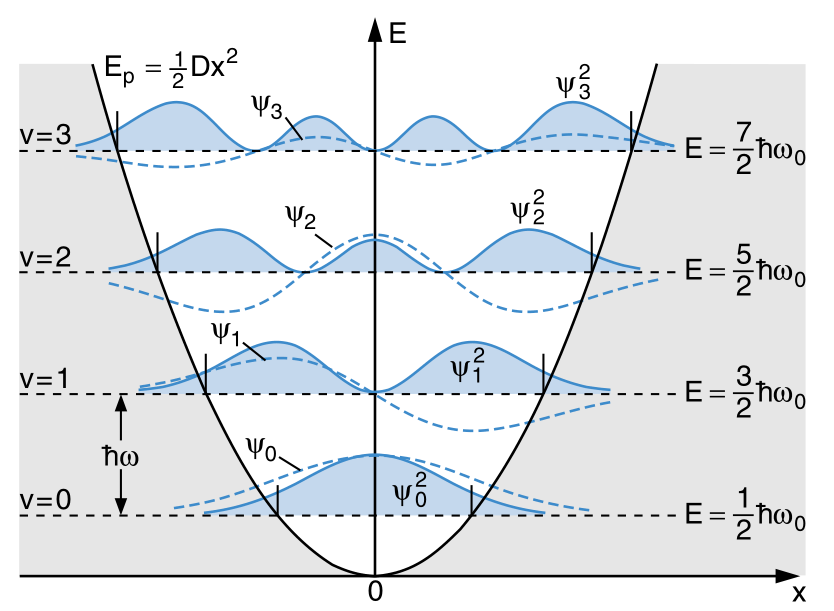
\includegraphics[width=15cm]{pics/harmonic1}
\caption{Energy levels of the harmonic oscillator with its 
    related wavefunctions\cite{Demtroeder1}.}
\label{fig:harmonic1}
\end{figure}
This potential is of outstanding importance for our experiment,
since the real potential will be aproximated in a region near
the minimum with a harmonic potential. 
To a few problems we can find the analytical solution
to the schrödingerequation, but to most
of the problems we need to approximate the solution with regards to an analyical
solution which is given. In the following sections we will introduce
the time-independent Perturbationtheory and give an example with the 
anharmonic oscillator how such an approximation can take place.
\subsubsection{Timeindependent Perturbationtheory}
We are following~\cite{fliessbach2008quantenmechanik}.
Lets assume we know the Eigenvalues and -functions of a specific
Hamiltonoperator $\hat{H_0}$ of the
unperturbed system (we further assume the eigenspaces to be
seperable, so we have no degeneracy. The case of degeneracy
can be done analogously) 
, numbered with $n\in \mathbb{N}$:

\begin{equation}
\hat{H_0} |n\rangle = \epsilon_n |n\rangle 
\end{equation}
and now we search for the solution of the perturbated Hamiltonian:
\begin{equation}
    \hat{H}|\psi \rangle = E|\psi \rangle 
\end{equation}
by means of the initial Hamiltonian:
\begin{equation}
    \hat{H} = \hat{H_0} + \lambda \hat{V}
\end{equation}
where we perturbate the original Hamiltonian with the Potential
$\hat{V}$ and give an approximate Soluation as long as Perturbation
is not of the same order of magnitude as $H_0$. 
The next step will be to apply this to the anharmonic 
Oscillator in order to get an estimation about the energyeigenvalues.
At first we have introduced a new parameter $\lambda$, which is the 
strength of the perturbation; for $\lambda = 1$ we have the problem
we want to solve, for $\lambda = 0 $ we arrive at the unperturbed
problem. Now we can expand in this parameter:
\begin{align}
    E_n(\lambda) &= \epsilon_n + \sum_{\nu =1}^{\infty} \lambda^\nu
    E_{n,\nu} \\ 
    |\psi_n(\lambda)\rangle &=
    |n\rangle + \sum_{\nu =1}^{\infty} \lambda^\nu
    |\psi_{n,\nu}(\lambda)\rangle
\end{align}
As result the solutions we are looking for will become:
\begin{align}
    E_n &= \epsilon_n + E_{n,1} + E_{n,2} + \cdots\\ 
    |\psi_n \rangle &= |n\rangle + |\psi_{n,1} \rangle + \cdots 
\end{align}
We assume for now that this series is converging and plug it into
the Schrödingerequation:
\begin{equation}
    (\hat{H_0} + \lambda \hat{V})
   \left( |n\rangle + \sum_{\nu =1}^{\infty} \lambda^\nu
        |\psi_{n,\nu}(\lambda)\rangle \right) =
\epsilon_n + \sum_{\nu =1}^{\infty} \lambda^\nu
    E_{n,\nu}  
    \left( |n\rangle + \sum_{\nu' =1}^{\infty} \lambda^{\nu'}
        |\psi_{n,\nu'}(\lambda)\rangle \right) 
\end{equation}
Now we can impose that the different powers of $\lambda$ have to
match on both sides and receive a set of equations:
\begin{align}
    \hat{H_0} |n\rangle &= \epsilon_n |n\rangle\\
    \hat{H_0} |\psi_{n,1}\rangle + \hat{V}|n\rangle &=
    \epsilon_n |\psi_{n,1}\rangle + E_{n,1}|n\rangle \label{eq:dev1}\\
    \hat{H_0} |\psi_{n,2}\rangle + \hat{V}|\psi_{n,1}\rangle &=
    \epsilon_n |\psi_{n,2}\rangle + E_{n,1}|\psi{n,1}\rangle 
    + E_{n,2}|n\rangle \label{eq:dev2}\
\end{align}
This set of equations yield recursive the Solutions of $E_{n,1}$,
$E_{n,2}$ and so on. Now we expand these single Wavefunctions 
into the new basis of energyeigenfunctions $|m \rangle$ with $m\in 
\mathbb{N}$:
\begin{equation}
    |\psi_{n,1}\rangle = \sum_{m=1}^{\infty} a_{nm} |m \rangle
    \label{eq:psi_expansion}
\end{equation}
We can plug this expansion now into into equation~\eqref{eq:dev1}:
\begin{equation}
    \sum_{m=1}^{\infty} (\epsilon_n - \epsilon_m) a_{nm} |m\rangle
    + E_{n,1} |n\rangle = \hat{V}|n \rangle
\end{equation}
With the Projection onto the dual eigenstate $\langle k|$ we can
use the orthonormality $\langle k | m \rangle = \delta_{m,k}$ 
of the energyeigenfunctions:
\begin{equation}
     (\epsilon_n - \epsilon_k) a_{nk} 
     + E_{n,1}\delta_{n,k}  = \langle k |\hat{V}|n \rangle
\end{equation}
For the case $k = n$ we get:
\begin{equation}
    E_{n,1} = \langle k |\hat{V}|n \rangle
\end{equation}
and for $k\neq m$:
\begin{equation}
    a_{n,k} = \frac{\langle k |\hat{V}|n \rangle}
    {\epsilon_n - \epsilon_k} \label{eq:a_nk}
\end{equation}
Equation~\eqref{eq:a_nk} together with~\eqref{eq:psi_expansion} 
gives us now:
\begin{equation}
    |\psi_{n}\rangle = |n\rangle + \lambda \sum_{m\neq n}^{\infty}
    \frac{\langle m |\hat{V}|n \rangle}{\epsilon_n - \epsilon_m}  
    |m \rangle + \lambda a_{n,n} + \mathcal{O}(\lambda^2)
\end{equation}
Now we can set $a_{n,n}=0$ (see footnote~\footnote{
Again we can use orthonormality:
\begin{equation*}
    1\overset{!}{=} \langle \psi_n|\psi_{n}\rangle 
    = \left | 1 + \lambda a_{nn} \right |^2 + \lambda^2
    \sum_{m\neq n}^{\infty}
    \left | \frac{\langle m |\hat{V}|n \rangle}
        {\epsilon_n - \epsilon_m} \right |^2 = 
    1 + \lambda (a_{n,n} + a^*_{n,n}) + \mathcal{O}(\lambda^2)
\end{equation*}
When $\lambda > 0 $ this results into:
\begin{equation*}
    a_{n,n} + a^*_{n,n} = 0 \Rightarrow \Re  [a_{n,n}] = 0
\end{equation*}
Since the Wavefunctions 
are invariant with respect to a phase $\phi$,
we can set without limitations $a_{nn}$ to zero.} for
further details) and we arrive
at:
\begin{equation}
    |\psi_{n}\rangle = |n\rangle + \lambda \sum_{m\neq n}^{\infty}
    \frac{\langle m |\hat{V}|n \rangle}{\epsilon_n - \epsilon_m}  
    |m \rangle  + \mathcal{O}(\lambda^2)
\end{equation}
For the Energy we can make use of the third equation and go to
the second order:
\begin{equation}
|\psi_{n,2}\rangle  = \sum_{m=1}^{X} b_{n,m} |m \rangle 
\end{equation}
We can plug this analogously into equation~\eqref{eq:dev2} and
arrive at:
\begin{equation}
 \sum_{m}^{\infty} (\epsilon_n - \epsilon_m) b_{nm} |m\rangle +
 \sum_{m}^{\infty} E_{n,1} a_{n,m} |m \rangle + E_{n,2} |n \rangle =
 \sum_{m}^{\infty} a_{n,m} \hat{V} |m \rangle
\end{equation}
Where again we use the orthonormality. For $k=n$ we get:
\begin{equation}
    E_{n,2} = \sum_{m}^{\infty} a_{n,m} \langle n |\hat{V}|m\rangle
= \sum_{m\neq n}^{\infty}\frac{|\langle n | \hat{V} | m \rangle |^2}
    {\epsilon_n - \epsilon_m}
\end{equation}
For $k\neq n$ we would arrive at the explicit formula for $b_{n,m}$
but this is not necessary for the further computations.
As final result we therefore get:
\begin{align}
    E_n &\approx \epsilon_n + \langle n|\hat{V} | n \rangle +
\sum_{m\neq n}^{\infty}\frac{|\langle n | \hat{V} | m \rangle |^2}
    {\epsilon_n - \epsilon_m} \\
    |\psi_n \rangle &\approx 
    |n\rangle + \sum_{m\neq n}^{\infty}
    \frac{\langle m |\hat{V}|n \rangle}{\epsilon_n - \epsilon_m}  
    |m \rangle 
\end{align}
\subsection{The anharmonic oscillator}
Lets assume we have solved the harmonic oscillator with 
\begin{align}
    \hat{H_0} &= \frac{\hat{p}^2}{2m} 
    + \frac{1}{2} m \omega_0^2\hat{x}^2 \\
    \hat{H_0}|n \rangle &= \epsilon_n |n \rangle \\
    \epsilon_n &= \hbar \omega_0 \left (n+ \frac{1}{2} \right)
\end{align}
Now perturbe this system with a kubic potential potential:
\begin{equation}
\hat{V} =\lambda \hat{x}^3
\end{equation}
Hence we can use the perturbation theory in linear order.
Since the parity of $\hat{V}$ is odd, the expectation value has 
to be zero:
\begin{equation}
    E_{n,1} = \lambda \langle n | \hat{x}^3 | n \rangle = 0 
\end{equation}
The wavefunctions have to be corrected as follows:
\begin{equation}
    |\psi_{n,1} \rangle = \sum_{m\neq n}^{\infty}
    \frac{\langle m |\hat{V}|n \rangle}{\epsilon_n - \epsilon_m}  
    |m \rangle 
    = \frac{\lambda}{\hbar \omega}
    |\psi_{n,1} \rangle = \sum_{m\neq n}^{\infty}
    \frac{\langle m |\hat{x}^3|n \rangle}{\epsilon_n - \epsilon_m}  
    |m \rangle 
\end{equation}
Now we have to calculate the matrix elements. Therefore we
introduce the creation- and annihilationoperator 
which are defined by $\hat{x}$:
\begin{equation}
    \hat{x} = \sqrt{\frac{\hbar}{2m\omega}}(\hat{a}^\dagger +
        \hat{a})
\end{equation} 
Now we can calculate iteratively the matrixelements
\footnote{
    Here we make use how $\hat{a}$ and $\hat{a}^\dagger$ act 
    on the eigenfunctions $|n\rangle$:
\begin{align*}
    \hat{x}|n'\rangle = \sqrt{\frac{\hbar}{2m\omega}}
    \left ( \sqrt{n' + 1}|n'+1\rangle 
        + \sqrt{n'}|n' - 1 \rangle \right ) 
\end{align*}
Applying once more:
\begin{align*}
\hat{x}^2|n'\rangle = \frac{\hbar}{2m\omega}
\left ( \sqrt{(n' + 1)(n' + 2)}|n'+2\rangle 
            + (2n' + 1) |n' \rangle
            + \sqrt{(n'(n'-1)}|n' - 2 \rangle \right ) 
\end{align*}
And applying for the third time:
\begin{align*}
    \hat{x}^3|n'\rangle &= \sqrt[3]{\left (\frac{\hbar}{2m\omega}\right )^2}
( \sqrt{(n' + 1)(n' + 2)(n'+3)}|n'+3\rangle 
    + 3 \sqrt{(n'+1)^3}|n' +1 \rangle  \\
 &+ 3 \sqrt{(n')^3}|n' -1 \rangle   
            + \sqrt{(n'(n'-1)(n'-2)}|n' - 3 \rangle  ) 
\end{align*}
Now this yields the matrixelements which we need:
\begin{align}
    \langle n | \hat{x}^3 | n' \rangle &=  
    \sqrt{\left (\frac{\hbar}{2m\omega}\right)^3}
( \sqrt{(n' + 1)(n' + 2)(n'+3)}\delta_{n,n'+3} 
    + 3 \sqrt{(n'+1)^3}\delta_{n,n'-1}  \\
    &+ 3 \sqrt{(n')^3}\delta_{n,n'-1}   
    + \sqrt{(n'(n'-1)(n'-2)}\delta_{n,n'-3}  ) 
\end{align}

}. After applying the justified indices, since only $n'=n\pm 1$ and
$m = n \pm 3 $ are not zero, we arrive at:
\begin{equation}
\begin{aligned}
    |\psi_{n,1} \rangle &= \frac{\lambda}{\hbar \omega}
    \sqrt{\left(\frac{\hbar}{2m\omega}\right)^3}
    ( -\frac{1}{3}\sqrt{(n + 1)(n + 2)(n+3)}|n+3\rangle 
    - 3 \sqrt{(n+1)^3}|n +1 \rangle  \\
 &+ 3 \sqrt{(n)^3}|n -1 \rangle  
    +\frac{1}{3} \sqrt{(n(n-1)(n-2)}|n - 3 \rangle  ) 
\end{aligned}
\end{equation}
We can also calculate the energy corrections:
\begin{equation}
    E_{n,2} = \langle n | \hat{V} | \psi_{n,1} \rangle 
    = \lambda \langle n | \hat{x}^3 | \psi_{n,1} \rangle 
\end{equation}
Which yields:
\begin{equation}
\begin{aligned}
    E_{n,2} &= \frac{\hbar^2 \lambda^2}{2 m^3 \omega ^4}
    \left[-\frac{1}{3}(n+1)(n+2)(n+3)
        -9(n+1)^3 + 9n^3 + \frac{1}{3}n(n-1)(n-2)
        \right ] \\
    &= -\frac{\hbar^2 \lambda^2}{2 m^3 \omega ^4}
    \left[ 30n^2+ 30n + 11 \right ]\\
    &= -\frac{30 \hbar^2 \lambda^2}{2 m^3 \omega ^4}
    \left[\left(n + \frac{1}{2} \right)^2 + \frac{11}{30} \right ]\\
\end{aligned}
\end{equation}
If we had a look at the closed form for all orders, we would
notice the possibility to expand the Energy Difference in terms
of powers of the original Energy $(n+\frac{1}{2})$ which we will
state here without proof:
\begin{equation}
    E_n = \hbar \omega_{0,0} \left(n + \frac{1}{2} \right) 
    - \hbar \omega_{0,1} \left(n + \frac{1}{2} \right)^2  
    + \hbar \omega_{0,2} \left(n + \frac{1}{2} \right)^3  
    + \cdots
\end{equation}
We did not include the small derivation independent of $n$,
since we will look only at energydifferences. Notice that
the final result is only valid for a small, odd Perturbation. 
\subsubsection{Energylevels and Wavefunctions
    of two-atomic molecules}

First we will write down the full Equations of the two-atomic
molecule and investigate after which parts we can further
simplify (This whole derivation will follow \cite{staatsexamen}):
\begin{equation}
        \hat{H}\psi = E\psi 
\end{equation}
Where we can expand the Hamiltonian in the position-space,
where we already split into the electrons ($i$) and the 
two nucleons $A$ and $B$:
\begin{equation}
    \hat{H} = \frac{-\hbar^2}{2} 
        \underbrace{\left(
        \sum_{i}{\frac{\nabla_i^2}{m_e}}
        +\frac{\nabla_A^2}{M_A} +\frac{\nabla_B^2}{M_B}
\right)}_{
\substack{\text{kinetic energy}\\\text{of electrons and nucleons}}}
+ \underbrace{\sum_{i>j}{\frac{e^2}{|r_i - r_j|}}
    }_{\substack{\text{potential energy}\\\text{electron-electron}}}
 - \underbrace{\sum_{i}{\frac{Z_A e^2}{|r_i - r_A|}}
 }_{\substack{\text{potential energy}\\\text{electron-nucleon $A$}}}
 - \underbrace{\sum_{i}{\frac{Z_B e^2}{|r_i - r_B|}}
 }_{\substack{\text{potential energy}\\\text{electron-nucleon $B$}}}
 +  \underbrace{\frac{Z_A Z_B e^2}{|r_A - r_B|}
 }_{\substack{\text{potential energy}\\\text{nucleon $A$ - nucleon $B$}}}
\end{equation}
Now we split the electronsolutions and the nucleonsolutions such
that the solutions of the electrons change only little when the
distance of the nucleons change, which is known as the
\textsc{BORN-OPPENHEIMER}-Approximation \cite{staatsexamen}:
\begin{align}
    \psi &= \psi_E ( \cdots r_i \cdots) \psi_N(r_A, r_B) \\
    \hat{ H}_E\psi_E &= \left(- \sum_{i}{\frac{\hbar^2\nabla_i^2}{2m_e}}
    + \sum_{i>j}{\frac{e^2}{|r_i - r_j|}}
    - \sum_{i}\frac{Z_A e^2}{|r_i - r_A|}
    - \sum_{i}\frac{Z_B e^2}{|r_i - r_B|}
    + 
    \right ) \psi_E = 
 E_E \psi_E \\
 \hat{H}_N\psi_N &= \left (
 -\frac{\hbar^2\nabla_A^2}{2M_A} -\frac{\hbar^2\nabla_B^2}{2M_B}
    - \sum_{i}\frac{Z_A e^2}{|r_i - r_A|}
    - \sum_{i}\frac{Z_B e^2}{|r_i - r_B|}
 + \frac{Z_A Z_B e^2}{|r_A - r_B|}
 \right ) \psi_N
=  E_N \psi_N 
\end{align}
Where we fixed the positions for the Hamiltonian
of the electrons such that they are not included in the
wavefunction. The interaction between electrons and the nucleons
will not be neglected since the Wavefunctions $\psi_E$ are still
dependend of the distance between the nucleons $r$. 
\par
The obvious problem arises when trying to solve these equations,
since it is not possible without great difficulties. 
The next step is to build up trialsolutions of $\psi_E$, 
consisting of solutions when there is only one electron and a
nucleon. These solutions are called one-electron orbital wave
and will be abbreviated
with \textit{MO} (\textit{Molecule orbital}) and the trialsolutions
will be built up upon linear combinations of those
(\textit{Linear combinations of atomic orbitals} method,
\textit{LCAO}). This method was first introduced 1929 by 
Sir John Lennard-Jones and has to be used with caution, since
it is only in certain limits applicable. The parameters which
appear in these combinations can be constrained by 
expectationvalues measured in experiments.
Now we will turn our attention to the movement of nucleons.
Since in our case we only have two of them, we can perform 
a coordinatetransform to the normal coordinates with a fictional
nucleon with mass
\begin{equation}
    \mu = \frac{M_A M_B}{M_A + M_B}
\end{equation}
so that our new Schrödingerequation with the wavefunction of the
fictional nucleon will look like:
\begin{equation}
    \nabla^2 \psi_N + \frac{2\mu}{\hbar^2} 
    \left[ E - V(r) \right] = 0 
\end{equation}
The Laplaceoperator written in spherical coordinates will yield
the spherical harmonics as eigenfunctions, so we can use a 
seperational ansatz for our wavefunction:
\begin{equation}
    \psi_N(r,\theta,\rho) = \frac{1}{r} S(r)Y(\theta,\rho)
\end{equation}
with the corresponding
differentialoperator, where $J\in \mathbb{N}_0$
corresponds to the Quantumnumber of the total angular momentum:
\begin{equation}
    \frac{\partial}{\sin\theta \partial \theta}\left (\sin\theta
    \frac{\partial Y}{\partial \theta}\right ) +
\frac{1}{\sin^2\theta} \frac{\partial^2 Y}{ \partial\rho^2}
 + J(J+1)Y = 0
\end{equation}
Thus we can split the rest of the wavefunction into the 
radial component of the Operator:

\begin{equation}
    \frac{d^2 S}{dr^2} + \frac{2\mu}{\hbar^2}
\left ( E - V(r) - \frac{J(J+1)\hbar^2}{2\mu r^2} \right ) S =0 
\end{equation}

If there is no further degeneracy (for instance due to not
considered interactions like spin) we can in theory write
down the Energyeigenvalues in terms of the two Quantumnumbers
$nu$ and $J$:
\begin{equation}
    E = E_{\nu,J}
\end{equation}
Practically this is not possible, so we look at two extrem cases.
\paragraph{The rigid Rotator} is based on the approximation to
fix the range of the two nuclei ($r =$const.) and so we only
look at $V(r)=0$ and $\frac{S(r)}{r} = 1$. We immedeatly get
the solution (since the sphericalharmonics already resolved
the eigenvalues):
\begin{equation}
    E = \frac{J(J+1)\hbar^2}{2\mu r^2}
\end{equation}
\paragraph{The rotationless Oscillator} just neglects the terms
arising from rotation, which is, looking at the lengthscale of
the former calculated eigenvalues, not inopportune.
The Operator then becomes:
\begin{equation}
    \frac{d^2 S}{dr^2} + \frac{2\mu}{\hbar^2}
    \left ( E - V(r) ) = 0 \right )
\end{equation}
The Eigenfunctions and -values are now very dependent on the 
potential energy $V(r)$ which is until now not a known 
potential, because it includes the repulsion due to the
pauliprinciple of the electronorbits as well as the attraction
of the charges. Furthermore the physical nature of dissociation
of the two nucleons also has to be encoded into it.
It is not possible to solve the potential analytically, but 
we will start to write down the properties already known:
\begin{itemize}
        \item Pauliprinciple:
            $\lim\limits_{r \rightarrow 0}{V(r)} = \infty $
        \item Dissociated nucleons:
$\lim\limits_{r \rightarrow \infty}{V(r)} = const. $
\item Before the Dissociation: Attraction of the nucleons with
    the maximal attraction at $r_e$ and the Dissociationenergy
    $D_e$ defined by 
    $ \lim\limits_{r \rightarrow \infty}{V(r)} - V(r_e)=: D_e$ 
\end{itemize}
The idea is now to capture this properties into the coefficients
of the taylored Potential and by doing so resolving the principle
physical behavior:
\begin{equation}
    V(r) = V(r_e) 
   + \frac{\partial V(r)}{\partial r}|_{r=r_e}(r - r_e)
   + \frac{\partial^2 V(r)}{2!\partial r^2}|_{r=r_e}(r - r_e)^2
   + \frac{\partial^3 V(r)}{3!\partial r^3}|_{r=r_e}(r - r_e)^3
   + \cdots
\end{equation}
As first approximation for energies near the minimum $r=r_e$ we
can finally use the harmonic potential. The constant term
$V(r_e)$ can be dropped since we are only interested in 
potential differences.
\begin{equation}
    V_{harm}(r) =
    \frac{\partial^2 V(r)}{2\partial r^2}|_{r=r_e}(r - r_e)^2
    =: \frac{k_e}{2}(r-r_e)^2
\end{equation}
Following this approach we can use the energyeigenvalues of the
harmonic oscillator in order to approximate
the vibrational states $\nu$:
\begin{equation}
    E_\nu =\sqrt{\frac{k_e}{\mu}}\hbar \left (\nu
        + \frac{1}{2}\right )
\end{equation}
In order to chose a more convenient unit we transform this
equation into $cm^{-1}$:
\begin{equation}
    G_{harm}(\nu) = \frac{E}{hc} = \omega_0 (\nu + \frac{1}{2})
    \quad \text{with the frequency} \quad
    \omega_0 = \frac{1}{2\pi c} \sqrt{\frac{k_e}{\mu}}
\end{equation}
The wider we leave the regime around $r_e$, speaking about 
higher vibrational states, the worse approximation with a harmonic
oscillator becomes. Qualitatively this is the case when energies
come nearer to the dissociation energy. An adhoc solution is 
to treat this with the already mentioned perturbationtheory in such
a way that we use the condition
\begin{equation}
    \frac{\partial V(r)}{\partial r}|_{r=r_e}        \gg
    \frac{\partial^2 V(r)}{2!\partial r^2}|_{r=r_e}  \gg
    \frac{\partial^3 V(r)}{3!\partial r^3}|_{r=r_e}  
    \cdots
\end{equation}
and can therefore justify the Ansatz:
\begin{equation}
    G(\nu) = \omega_e (\nu + \frac{1}{2} ) 
    - \omega_e x_e (\nu + \frac{1}{2} ) ^2 
    + \omega_e y_e (\nu + \frac{1}{2} ) ^3 
    - \omega_e z_e (\nu + \frac{1}{2} ) ^4 
    + \cdots 
\end{equation}
Since in the experiment it is clearly impossible to seperate
the incoming higher frequencies, we will treat $\omega_e x_e$ as 
one variable, similarily to the others, where they also connected
on lengthscales by
\begin{equation}
    \omega_e \gg \omega_ex_e \gg \omega_e y_e \cdots 
\end{equation}
As before we can shift the equations to make them more convenient,
in this case to scale them to the zeroenergy
\begin{equation}
    G \mapsto G_0 := \left [G-G(0) \right ] 
        \quad \text{which is given by}
    \quad G(0)=\frac{1}{2}\omega_e - \frac{1}{4}\omega_e x_e 
    + \frac{1}{8} \omega_e y_e + \cdots 
\end{equation}
So we get for the shifted term:
\begin{equation}
    G_0(\nu) = 
\end{equation}
\clearpage



\section{Setup and procedure}
First we give an overview of the program which constitutes the experiment. In another subsection, 
we give a describtion of the setup used. 
\subsection{Procedure}
The procedure of measurements consists of the following six points:
\begin{enumerate}
    \item 
        \textbf{Assessing the detectors and probe at hand with the oscilloscope:}
        We measure the signals of the preamplifier (PA) as wel as uni- and bipolar outputs of 
        main amplifier (MA) at the oscilloscope. With this signal, we calculate the ascending time 
        of the signal.
    \item 
        \label{it:task2}
        \textbf{recording the energy spectrum of $^{57}$Co and $^{241}$Am:}
        The multichannel analyzer (MA) we measure the energy spectrum of both probes 
        for ca. 10 minutes. With the $^{57}$Co sample, we test the sensibility of each detector
        and the optimal positioning of the sample (which is not symmetric). After assigning the 
        channel-energy relationship based on the knowledge of some peaks, we interprete the other visible peaks.
    \item
        \textbf{setting the energy windows:}
        In this step, we restrict the events passed by the single channel analyzer (SCA) to those 
        of the 14.4 keV and 122 keV photons, respectively.
    \item
        \textbf{measuring the delayed coincidences:}
        Using the Time-to-Amplitude converter (TAC), we record the delays between 14.4 keV and 122 keV 
        events. Since the 14.4 keV photon is only emitted in 10 \% of the cases, we use this signal to start the 
        TAC, and stop with the delayed 122 keV photon, expecting to drastically reduce the dead time of the 
        measurement.
    \item
        \textbf{measuring the background (random coincidences):}
        Taking out the delay of the 122 keV signal and further introducing a delay on the 14.4 keV signal, 
        we measure the background. 
    \item
        \textbf{time calibration of Time to Amplitude converter (TAC):}
        In order to correlate measured channel and the respective time delay, we measure the channel 
        assigned by TAC and MCA corresponding to a known delay and perform a fit a linear function between 
        the two quantities. This correspondance will be used in the anaylsis of the delayed coincidences. 
\end{enumerate}


\subsection{Experimental setup}
The setup of the experiment consists of a fixed part with probe and a detector at each side 
as well as a part with the electronics. The devices are adapted to each part, as described below. 

A photo of the two detectors and the probe is shown in figure \ref{fig:position_1}. The given setup also 
defines position 1, later referred to as "Pos1" (see table \ref{tab:config2}). Position 2 ("Pos2") corresponds 
to the probe rotated by $180^\circ$. From its geometry, one can already suspect that the number of photons 
that can be measured from either direction is not equal. A similar condition is true for the detectors:
Already on the first glance, it is clear that the two are not of the same model. In fact, the left detector 
is an older model and suspected to be less sensitive. A more quantitative statement will be made in the 
of the second part of the experiment (see \ref{it:task2}).

\begin{figure}[H]
    \centering
    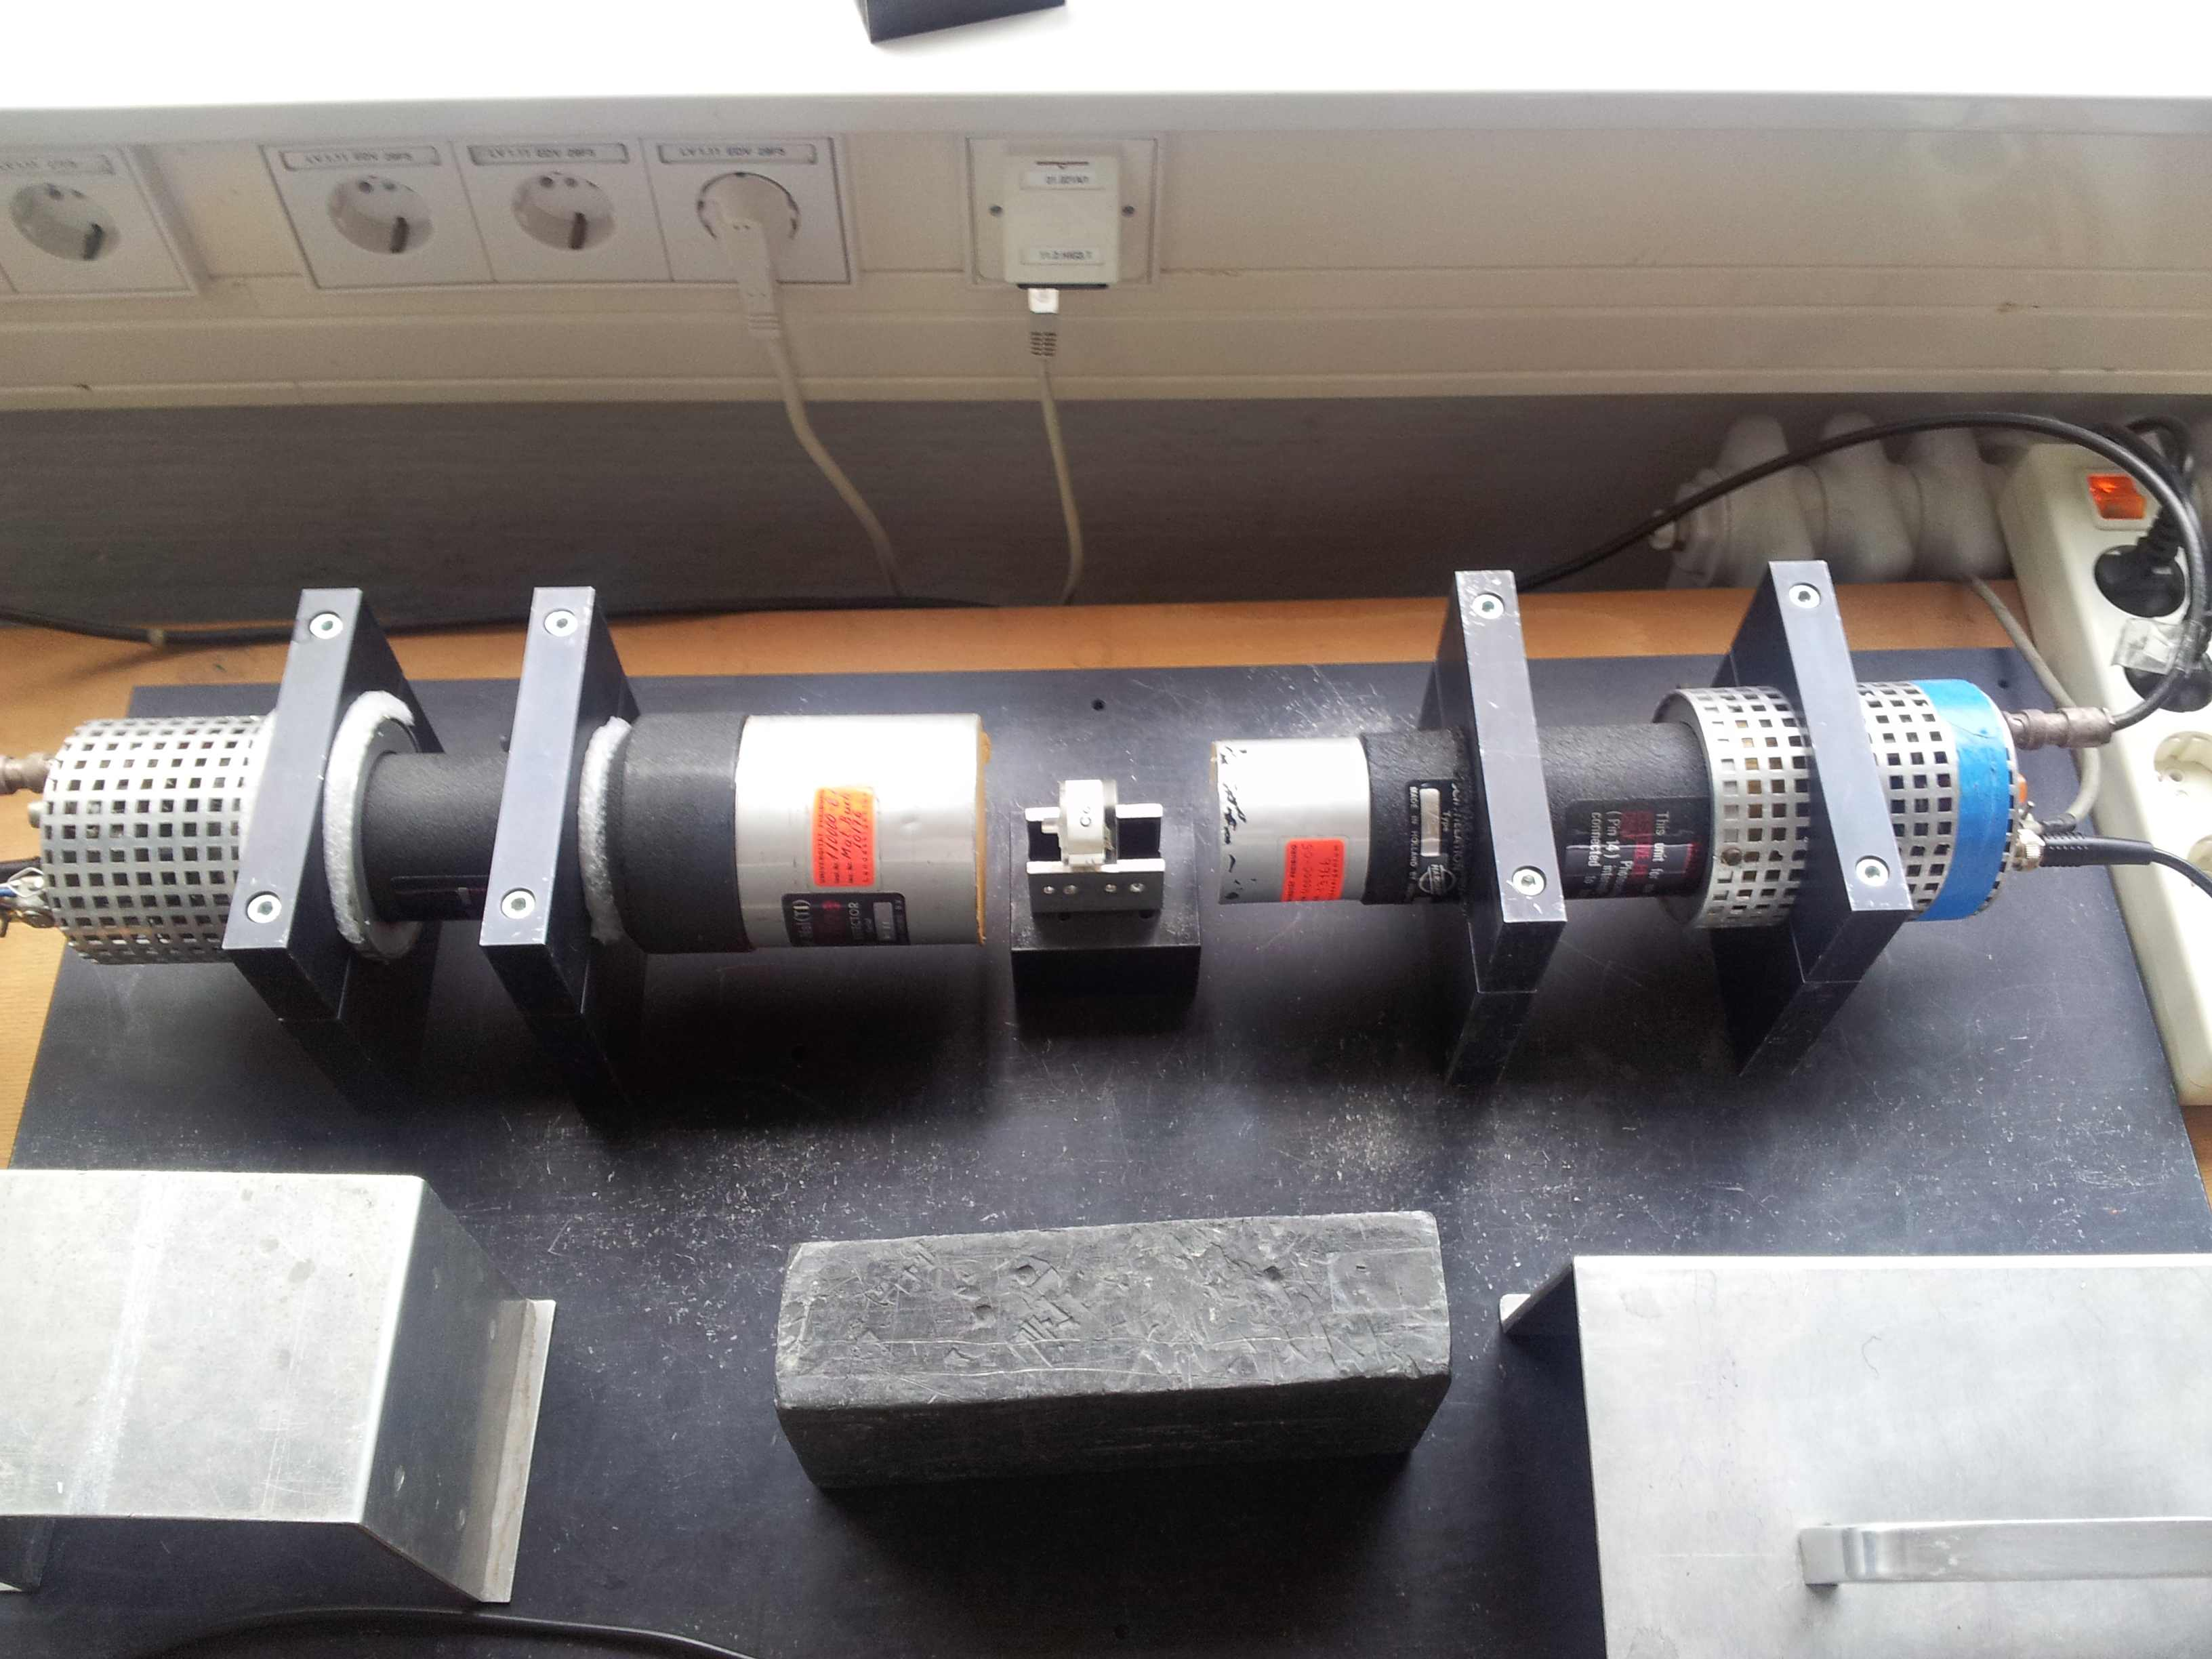
\includegraphics[width=0.8\linewidth]{figures/position_1.jpg}
    \caption{
        Photo of the $57$^Co probe and the two detectors with the setup used in the 
        experiment. The orientation of the probe is the one used for the measurement of 
        the delayed coincidences, with the larger opening facing the right detector. 
        During the measurements, the probe is isolated by the 
        }
    \label{fig:position_1}
\end{figure}




\newcommand{\figdir}{analysis/figures/}

\section{Evaluation}
\subsection{Techniques used in the evaluation}
All calculations in this section are done with scripts written in 
the \textit{python} programming language~\cite{python}, relaying in several 
packages:
\begin{itemize}
    \item
        \textit{matplotlib}~\cite{Hunter2007} for plotting,
    \item
        \textit{scipy}~\cite{scipy} for fitting, and 
    \item
        \textit{uncertainties}~\cite{uc} for error propagation.
\end{itemize}
The latter applies gaussian error propagation for correlated and uncorrelated variables. 
We will thus not explicitly write down the formulas for the error propagation 
for each quantity calculated but instead state the numerical result, only. 
We will, however make a quick remark on the use of covariance matrices in 
error propagation: Contrary to measured data, which in our case is usually 
expected to be uncorrelated, all fitted data yields variables that in general correlate. 
The propagation is then done as follows:
Let's assume we have random
variables $x_0,...,x_N$ which are correlated through the $N\times N$ Matrix $cov(x_i,x_j)$.
For a scalar function $f(x_0,...,x_N) \rightarrow \mathbb{R}$, the variance is estimated (linearly) by:
\begin{equation}
Var[f] = \sigma^2 = \sum_{i,j} \frac{\partial f}{\partial x_i} \frac{\partial f}{\partial x_j} cov(x_i,x_j) \,.
\end{equation} 
If instead, $\mathbf{f}$ is a vector field in $m$ dimensions, namely 
$\mathbf{f}(x_0,...,x_N) \rightarrow \mathbb{R}^m$, then the components of $\mathbf{f}$ 
are further correlated. We can write down the relation between the covariance matrices $V$ and $U$ of 
$\mathbf{x}$ and $\mathbf{f}$, respectively, in matrix relations:
\begin{equation}
    U = A V A^T
\end{equation}
where $A$ is the matrix defined by 
\begin{equation}
    A_{ij} = \left[ \frac{\partial f_i}{\partial x_j}\right]_{\mathbf{x} = \mathbf{\mu}}
\end{equation}
with expectation value $E[\mathbf{x}] = \mathbf{\mu}$.~\cite{cowan1998statistical}
In order to facilitate notation, the covariance matrices will in general be notated without 
specifying the units. If not specified explicitly, the units will correspond to those of the
variables: If $x_i, x_j$ have the units $[x_i], [x_j]$, respectively, 
then the entry of the covariance matrix has the unit $[x_i] * [x_j]$. 

\subsection{Lattice constant of sine grating}
Observing the intensity on the screen, we noticed that the beam was not 
diffracted in the plane $y = \mathrm{const.}$ (where y denotes the horizontal direction). 
We thus notated the coordinates on the graph paper. The measured values 
are displayed in table \ref{tab:sine_distances}. The estimated error of 
$s_{xy} = 1$ mm in both directions mainly stems from the fact that the edge of the beam 
has only a limited sharpness. 
\renewcommand{\arraystretch}{1.5}
\begin{table}[htdp]
    \centering
    \begin{tabular}{|p{6.18cm}|p{3.82cm}|p{3.82cm}|}
        \hline
        \rowcolor{tabcolor}
        Maximum & $x$ / mm & $y$  / mm \\ \hline
        $0.$        & 3     & 3\\
        $1.$, left & 48    & -1\\
        $1.$, right  & -42   & 7\\
        \hline
    \end{tabular}
    \caption{
        Measurements of positions of maxima for the sine amplitude grating. 
        The error is estimated to be $s_{xy} := s_x = s_y = 1$ mm. 
        }
    \label{tab:sine_distances}
\end{table}
The distance $d_\mathrm{sin}$ between the zeroth and first maximum is calculated by taking half of 
the distance between the two first maxima:
\begin{align}
    d_\mathrm{sin}   &= \frac{1}{2} \sqrt{(x_l - x_r)^2 + (y_l - y_r)^2} = 45.1 \mathrm{mm} \\
    \begin{split}
        s_{d_\mathrm{sin}} &= \sqrt{\sum{
                \left(\frac{\partial d_\mathrm{sin}}{\partial x_i}\right)^2 s_{x_i}  + 
                \left(\frac{\partial d_\mathrm{sin}}{\partial y_i}\right)^2 s_{y_i} 
                }} \\
        &= \frac{s_{xy}}{\sqrt{2}} \\
        &= 0.7 \, \mathrm{mm}\, ,
    \end{split}
\end{align}
where $x_r, x_l$ and $y_r, y_l$ correspond to the coordinates of right and left 
maximum, respectively and $s_{d_\mathrm{sin}}$ denotes the error calculated by gaussian error propagation.
The distance between screen and grating was $l_\mathrm{sin} = (56 \pm 2)$ mm. By geometric construction, 
we can identify the angle $\theta$ between the lines connecting grating and the maxima 
of zeroth and first order on the screen, respectively. Using further the 
necessary condition for positive interference (see eqn \eqref{eq:inter_cond} in the theory section), 
we calculate the lattice constant $K_\mathrm{sin}$ for the sine grating:
\begin{align}
    \sin(\theta)&= \frac{d_\mathrm{sin}}{\sqrt{l_\mathrm{sin}^2 + d_\mathrm{sin}^2}} \\
    \sin(\theta)&= \frac{m\lambda}{K_\mathrm{sin}} \\
    \Rightarrow \qquad 
    K_\mathrm{sin}    &= m \lambda\sqrt{\left(\frac{l_\mathrm{sin}}{d_\mathrm{sin}}\right)^2 + 1} 
        = (1.01 \pm 0.02) \, \mu\mathrm{m}
\end{align}
Although no nominal value is stated, the measured value suggests, that the grating has been 
constructed to a nominal value of $K_\mathrm{sin, nom} = 1$ $\mu$m. 

\subsection{Calibration}
For all further measurements, we needed to calibrate the setup and use the gauge gratings 
to establish the relationship between the signal observed on the oscilloscope and the 
actual distance between the peaks which would be observed on a screen at the position of diode~1. 
For this part, we set the lenses such that the beam would be widened and collimated. We tested the collimation 
with the graph paper. The measured distances can be seen in the handwritten records, see appendix \ref{sec:records}.
The small focal length of lens~3 ($f_3 = 300$ mm) made it impossible to focus the beam exactly onto diode~1. We 
chose the closest position allowed by the setup, such the lens would not interfere with the second beam. 
We were told not to change the positions of the diodes. 

We measured the peaks with the amplitude grating two times, since we noticed a difference when turning the grating. 
Both measurements are plotted in figure \ref{fig:calibrate_peaks}. 
We searched for the times at the maxima numerically, taking the center value in case of a plateau. 
The results are plotted as dotted lines. We relinquish the displaying of all numerical interim results. 
The error was estimated somewhat bigger then the calculated standard deviation (in almost 
    all cases, $s_{\overline{t_\mathrm{max, calculated}}}  = 0.004$ ms), which has little meaning, 
since we only took two measurements. The estimated errors are then further propagated for the fits. 

\renewcommand{\arraystretch}{1.5}
\begin{table}[htdp]
    \centering
    \begin{tabular}{|p{3cm}|p{2cm}|p{2cm}|p{2cm}|}
        \hline
        \rowcolor{tabcolor}
        Maximum & $t_1$ / ms & $t_2$  / ms & $\overline{t_\mathrm{max}}$ / ms \\ \hline
        $3.$, left  & 0.204     & 0.211 & 0.207 \\
        $2.$, left  & 0.298     & 0.306 & 0.302 \\
        $1.$, left  & 0.393     & 0.400 & 0.397 \\
        $0.$,       & 0.489     & 0.496 & 0.492 \\
        $1.$, right & 0.585     & 0.591 & 0.588 \\
        $2.$, right & 0.682     & 0.686 & 0.684 \\
        \hline
    \end{tabular}
    \caption{
        Peaks for the calibration grating. We estimate the error on each 
        value of $\overline{t_\mathrm{max}}$ with 
        $s_{\overline{t_\mathrm{max}}} = 0.01$ ms for all maxima except the 
        very small peak for $m = 2$ on the right side ($s = 0.04$).
        }
    \label{tab:calibrate_peaks}
\end{table}
\begin{figure}[htpb]
    \centering
    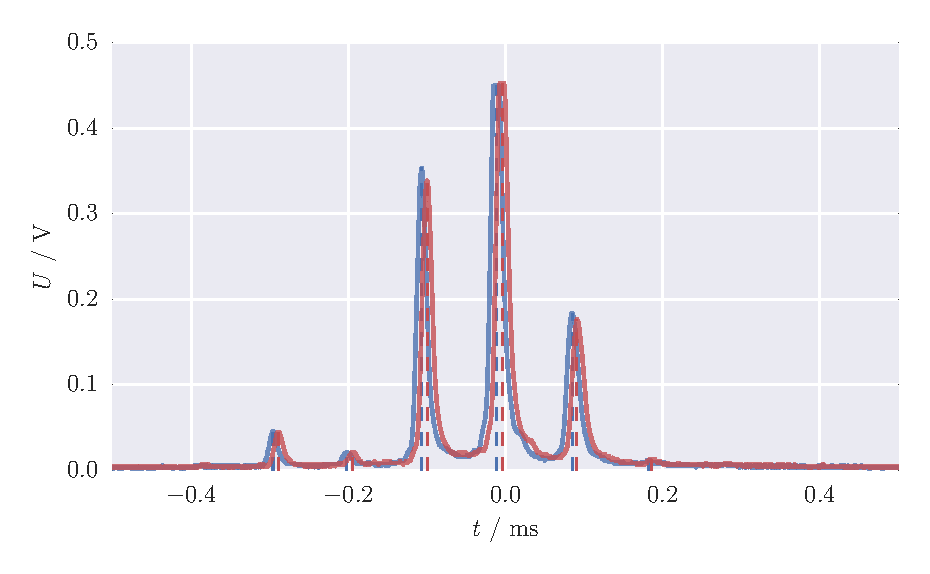
\includegraphics[width=1.0\linewidth]{figures/calibrate_peaks}
    \caption{
        Measured signal for the gauge gratings, each corresponding to a different orientation of the 
        grating. The maxima are found numerically, taking the central value in case of a plateau. 
        The is a clear offset of the maxima corresponding to the same order. For further calculations, 
        we take the mean value of the two. 
        }
     \label{fig:calibrate_peaks}
\end{figure}

From the maxima, we could calculate the linear correspondence $\theta(t)$, 
which is derived by \ref{eq:N_lines_interference}:
\begin{equation}
    \theta(m) = \arcsin\left(\frac{m \lambda}{K}\right)
\end{equation}
Since the mirror rotates with constant angular speed $\omega$, we can 
also write $\theta(t) = \omega t + \theta_0$. By correctly identifying the maxima, and using the 
known lattice constant $K_\mathrm{gauge}$ of the gauge grating, we can perform a linear fit.
The result is plotted in figure \ref{fig:calibrate_fit}. The values and the corresponding 
covariance matrix are: 
\begin{align}
    \omega &= 0.0663 \, \mathrm{rad / s}\\
    \theta_0 &= 0.0005 \, \mathrm{rad} \\
	\mathrm{cov} &=
	\begin{pmatrix}
		2.0\mathrm{e}-07 &-6.1\mathrm{e}-09 \\
		-6.1\mathrm{e}-09 &6.0\mathrm{e}-09 \\
	\end{pmatrix} 
\end{align}
The standard deviation $\sigma_\omega$ of the relevant parameter $\omega$ is only about 
\begin{equation}
    \sigma_\omega / \omega = \frac{\sqrt{2.0 * 10^{-7}}}{0.0663} \approx 0.7 \% \, .
\end{equation}
This small error is linked to the constant rotational speed 
one could expect of the motor. The correlation of $\omega$ to $\theta_0$ is of one magnitude smaller 
than the variance - the effect could thus be neglected in the further calculations (although we keep 
    on using the correlated variables).

\begin{figure}[htpb]
    \centering
    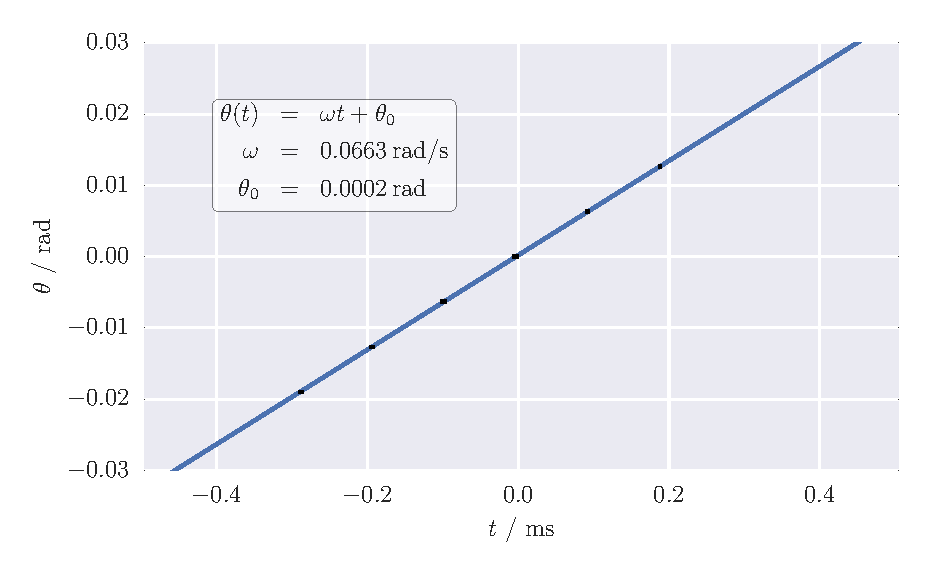
\includegraphics[width=1.0\linewidth]{figures/calibrate_fit}
    \caption{
        Fit of the angles identified for the gauge grating with known 
        lattice constant of $K = 10,000$ lines/m. The errors on the time corresponds to the
        shift observed when turning the grating around. The fit is drawn with the errors obtained 
        by error propagation using the corresponding covariance matrix.
        }
    \label{fig:calibrate_fit}
\end{figure}

\subsection{Lattice constant and resolution for five gratings}
Using $\theta(t)$, we can calculate the lattice constants for the five amplitude gratings. 
For that, we find the times corresponding to the $m$th maximum numerically. The width 
of the peaks is approximately equal at half maximum, such that we do not put weights 
on each maximum. We also neglect to fit gaussians on each peak. An application of such methods 
for this measurement does not increase the precision of the measurement to a appreciable degree, 
as the peaks in the measured data are already quite symmetric and the applied simpler method yields 
good results, at least in comparison with other errors. 
Plots of the measured data and the maxima can be found in the appendix, see 
\ref{fig:gratings_maxima}. 

We again apply the formula \ref{eq:N_lines_interference}. Since we use numerical computation, 
there is no need to do the first order approximation of the sine. The lattice constants are thus 
found by
\begin{equation}
    K_i = \frac{m\lambda}{\sin(\theta)}\, .
\end{equation}
One observes from the plotted data that only a finite number of maxima is seen and, more important, 
that some maxima of lower order than the highest maximum observable are not visible, either. 
Thus, assigning the maxima has to be done by hand, already assuming the almost equal distances between the 
maxima. In order to calculate the angle $\theta$, we translated the time $t_\mathrm{osci} \rightarrow t$ 
such that $t = 0$. 
This had to be done, as the oscilloscope did not save the time with respect to the trigger 
but set $t = 0$ to the first data point. 

\begin{table}[htdp]
    \centering
    	\begin{tabular}{|p{3.82cm}|p{6.18cm}|p{3.82cm}|}
		\hline
		\rowcolor{tabcolor}
		Grating & Orders visible & $\overline{K}$ / ($\mu$m)  \\ \hline
		$1$  & $-4, -3, -2, -1, 0, 1, 2, 3, 4$ & $ 125.8 \pm 2.5 $ \\
		$2$  & $-3, -2, -1, 0, 1, 2$ & $ 34.1 \pm 0.8 $ \\
		$3$  & $-5, -4, -2, -1, 0, 1, 2, 4, 5$ & $ 100.8 \pm 1.2 $ \\
		$4$  & $-5, -3, -1, 0, 1, 3, 5$ & $ 100.8 \pm 1.0 $ \\
		$5$  & $-2, -1, 0, 1, 2$ & $ 50.7 \pm 1.2 $ \\
		\hline
	\end{tabular}

    \caption{
        Calculated lattice constants of amplitude gratings one to five. 
        The orders $m$ have to be assigned by hand, as for grating 3 and 4 some 
        orders in between are missing. The error is the standard deviation of 
        the weighted mean.
        }
    \label{tab:gratings_K}
\end{table}

The resolution of the gratings can be calculated as described in the theory section, 
see equation \eqref{eq:resolution}.
The diameter $\phi$ of the laser in this experiment was measured with a slide gauge. 
\begin{equation}
    \phi = (2.9 \pm 0.5) \, \mathrm{mm}
\end{equation}
We approximate the number $N$ of lines illuminated by
\begin{equation}
    N = \phi / K
\end{equation}
with lattice constant $K$. The number of lines observed at full illumination and the
resulting resolution $a$ using the previously estimated lattice constants $\overline{K_i}$
are displayed in table \ref{tab:gratings_resolution}. During the experiment, the resolution was 
limited not only to the natural resolution of the gratings with the applied beam, but 
also due to the fact, that the trigger also passed diode 1, such that an observable peak
might have been overlapped by this signal. We restricted ourselves to use only those
directly visible, however. 

\begin{table}[htdp]
    \centering
    	\begin{tabular}{|p{2cm}|p{3.82cm}|p{3.82cm}|p{3.82cm}|}
		\hline
		\rowcolor{tabcolor}
		Grating & $n$ orders visible & $N$ lines illuminated & resolution $a$ \\ \hline
		$1$  & $10$ & $23.1 \pm 4.1$ & $ 230 \pm 40 $ \\
		$2$  & $6$ & $84.8 \pm 14.8$ & $ 508 \pm 88 $ \\
		$3$  & $10$ & $28.7 \pm 5.0$ & $ 287 \pm 50 $ \\
		$4$  & $9$ & $28.7 \pm 5.0$ & $ 258 \pm 44 $ \\
		$5$  & $6$ & $57.1 \pm 10.1$ & $ 342 \pm 60 $ \\
		\hline
	\end{tabular}

    \caption{
        Resolutions of five gratings for largest illumination possible 
        in the experiment (diameter of laser $\phi = 2.9 \pm 0.5\,$mm). 
        We used the lattice constants calculated before, \ref{tab:gratings_K}. 
        }
    \label{tab:gratings_resolution}
\end{table}

\subsection{Aperture function}
In this section we calculate the aperture function of grating 1 from the intensity 
of the maxima observed. This is done by approximating its Fourier series to the maximal 
order visible, as described in the theory section. The obtained data from the measurement 
shows asymmetry in most cases. The plotted data can be seen in the appendix, 
\ref{fig:aperture_positions_detail}. We chose position five for the further calculation, 
because it allows to identify maxima up to the fourth order on both sides. 
We obtained the intensities by taking the mean of each two values for one order. 
The intensities are listed in table \ref{tab:intensities} below.
The error on the channels of the oscilloscope 
\textit{Hameg HM1508-2} in the used resolution is given by
\begin{equation}
    S_U = 3 \% \times 1\mathrm{V} = 0.03 \textrm{V}
    \label{eq:error_osci}
\end{equation}
The affected data is usually the height of an absorption peak. It's
error is than taken to be $S_U$ with the corresponding height. 
Due to the dependency on the scale, we saved the data at two 
scales for the forgoing analysis -- one for the peaks of 
zeroth maximum, another for all higher orders, which in most cases
are much lower. 
\begin{table}[H]
    \centering
    	\begin{tabular}{|p{3.82cm}|p{3.82cm}|p{3.82cm}|p{3.82cm}|}
		\hline
		\rowcolor{tabcolor}
		Order $m$ & $I_\mathrm{left}$ / V & $I_\mathrm{right}$ / V & $\overline{I}$ / V  \\ \hline
		$0$ & 	 & 	& $1.53 \pm 0.06$ \\ 
		$1$ & $0.144 \pm 0.006$ & $0.140 \pm 0.006$ & $0.142 \pm 0.004$ \\ 
		$2$ & $0.120 \pm 0.006$ & $0.066 \pm 0.006$ & $0.093 \pm 0.004$ \\ 
		$3$ & $0.063 \pm 0.006$ & $0.025 \pm 0.006$ & $0.044 \pm 0.004$ \\ 
		$4$ & $0.024 \pm 0.006$ & $0.013 \pm 0.006$ & $0.019 \pm 0.004$ \\ 
		\hline
	\end{tabular}

    \caption{
        Intensities of the maxima in units of the oscilloscope for grating 1 at position 5. 
        For the aperture function, 
        these intensities are normalized. The zeroth maximum is simply the value obtained 
        from the graph, as no mean is formed. The errors are taken to be those of the
        oscilloscope.
        }
    \label{tab:intensities}
\end{table}
Using the intensities, we can calculate the aperture function. 
The result is plotted in figure \ref{fig:aperture_function}. 
The resulting approximation on the width of the slits is 
\begin{equation}
	b = (26.6 \pm 5.3)\, \mu\mathrm{m}
\end{equation}
where the error is approximated manually with $10\%$. The ratio between 
lattice constant and width can thus be calculated to 
\begin{equation}
	\frac{b}{K} = \frac{ 26.6 \pm 5.3 }{ 125.8 \pm 2.5 } = 0.21 \pm 0.04 \, .
\end{equation}
Since there are no specifications on the nominal values of the gratings, we cannot 
compare the obtained value of this ratio with other results. 


\begin{figure}
    \centering
    \begin{subfigure}[b]{\pltw}
        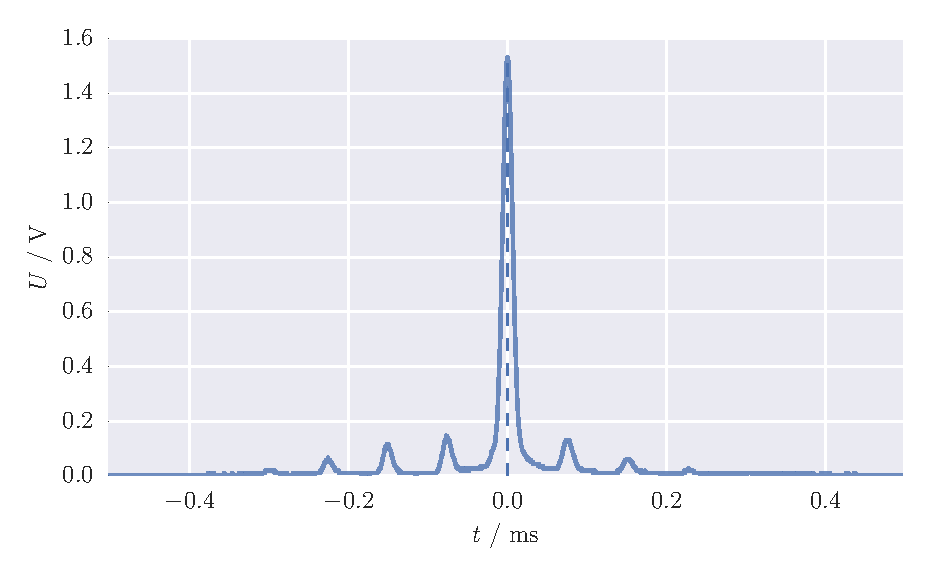
\includegraphics[width=\textwidth]{figures/aperture_5a}
        \caption{Position 1, scale for zeroth maximum}
        \label{}
    \end{subfigure}\quad
    \begin{subfigure}[b]{\pltw}
        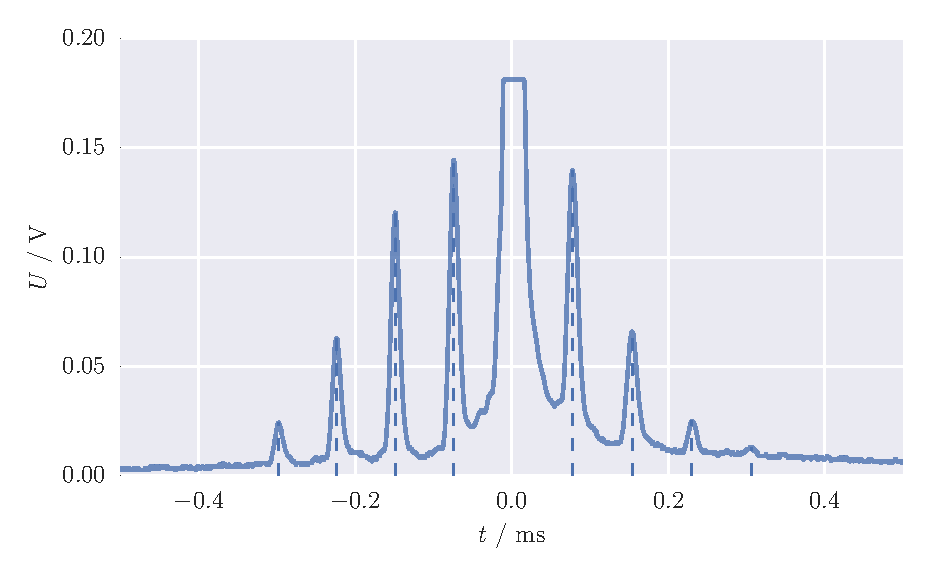
\includegraphics[width=\textwidth]{figures/aperture_5b}
        \caption{Position 1, scale for maxima with $m \neq 0$}
        \label{}
    \end{subfigure}
    \caption{
        Measured intensities for grating 1 for position 5. 
        For the calculation of the aperture function, 
        we take the mean value of both intensities of the same order. 
        }
    \label{fig:aperture_positions_detail}
\end{figure}
\begin{figure}
    \centering
    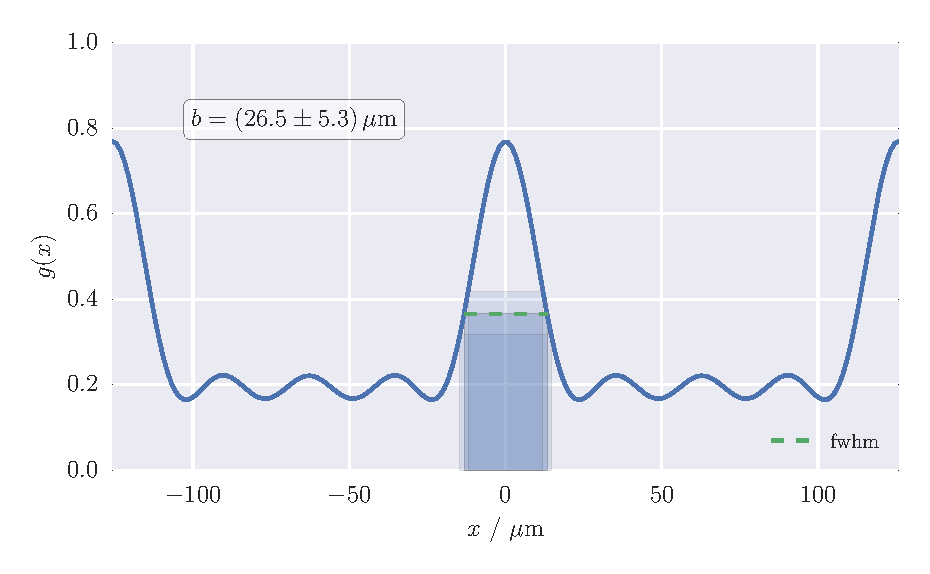
\includegraphics[width=\textwidth]{figures/aperture_function}
    \caption{
        Approximation of the aperture function, using its Fourier series up to the 
        4th order. The shaded area indicates the full width at half maximum (fwhm) 
        of the global maximum, which is taken as an approximation of the width of the 
        slits. The error $s_b$ is approximated by hand with a relative error of $10\%$. 
        indicated by the boxes with higher transparency. 
        }
    \label{fig:aperture_function}
\end{figure}
\FloatBarrier


\clearpage
\subsection{Ultrasonic evaluation}
As already stated we have measured the intensity distribution of the laser
passing through a phase grating, in particular the phase grating created
by ultrasonic waves passing through the medium. We evaluate these diffraction patterns
by determining the position of the maxima and their intensities with an algorithm
by extremal analysis. The results are seen in 
figure~\ref{fig:ultrasonic1}.
The error of this analysis
is given by the width of the respective peaks, the error on the amplitude is 
taken to be the error if the oscilloscope, as described before \eqref{eq:error_osci}.
The conversion from time to angle was given in the previous section (see
figure\ref{fig:calibrate_fit} for the conversion fit). In the following we 
will give all information in the captions of the figures and tables, respectively.
We will give the least square fits for the maxima from order zero to three and 
their coefficients along with the covariance matrices.

\begin{figure}[H]
    \centering
    \begin{subfigure}[b]{\picwidth}
        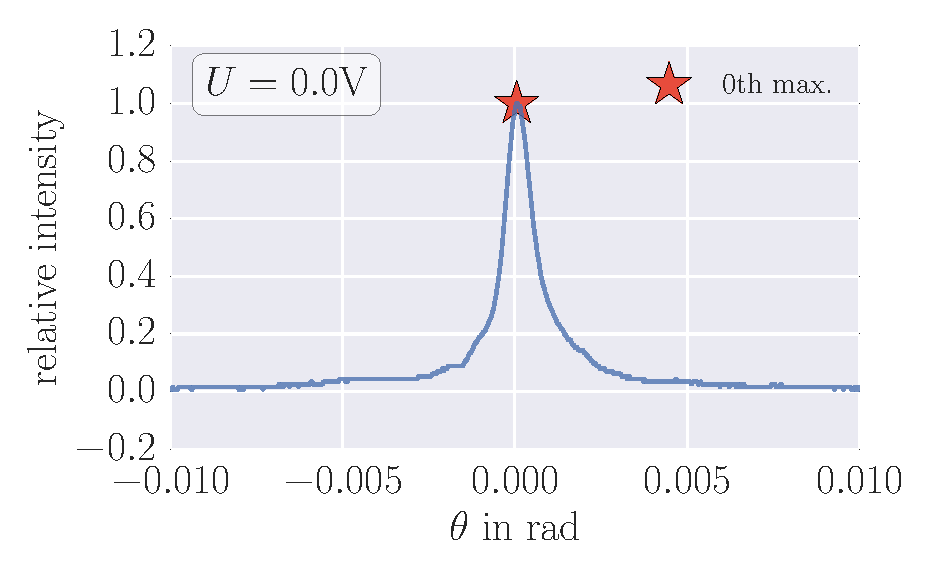
\includegraphics[width=1.0\textwidth]{analysis/figures/raman_001}
        \caption{}
        \label{fig:raman_001}
    \end{subfigure}
    \begin{subfigure}[b]{\picwidth}
        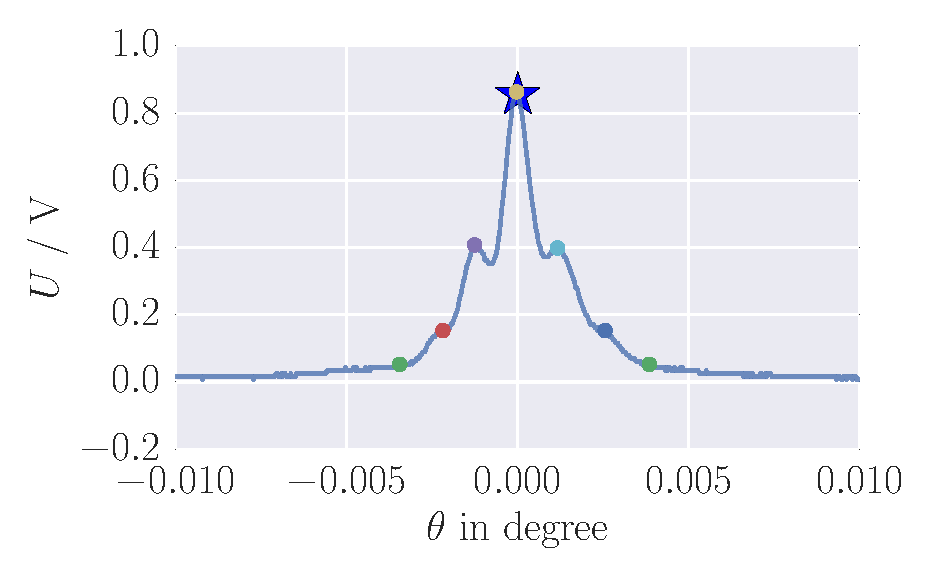
\includegraphics[width=1.0\textwidth]{analysis/figures/raman_007}
        \caption{}
        \label{fig:raman_007}
    \end{subfigure}
    \begin{subfigure}[b]{\picwidth}
        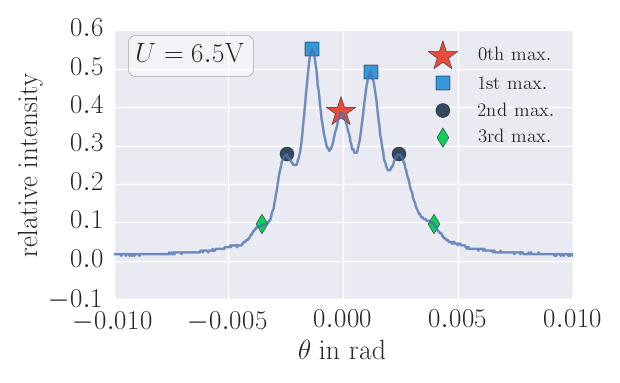
\includegraphics[width=1.0\textwidth]{analysis/figures/raman_014}
        \caption{}
        \label{fig:raman_014}
    \end{subfigure}
    \begin{subfigure}[b]{\picwidth}
        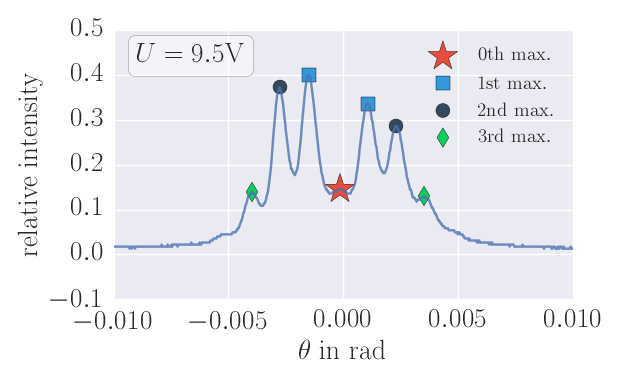
\includegraphics[width=1.0\textwidth]{analysis/figures/raman_020}
        \caption{}
        \label{fig:raman_020}
    \end{subfigure}
    \caption{
        These figures constitute a selection of the available measurements 
        from the ultrasonic experiment. We denoted the 
        different orders by different symbols (see the respective legends). 
        The maxima were estimated by an algorithm which seeks for local extrema
        and evaluates them with a certain threshold. The threshold is determined 
        by the minimal distance of maxima, estimated by the theoretical 
        relationship $sin(\theta) = m \lambda / \Lambda$. 
        The intensities are given by the measured voltage,
        normed by the zeroth maximum at $U=0V$.
        }
    \label{fig:ultrasonic1}
\end{figure}
\newpage
\begin{figure}
    \centering
    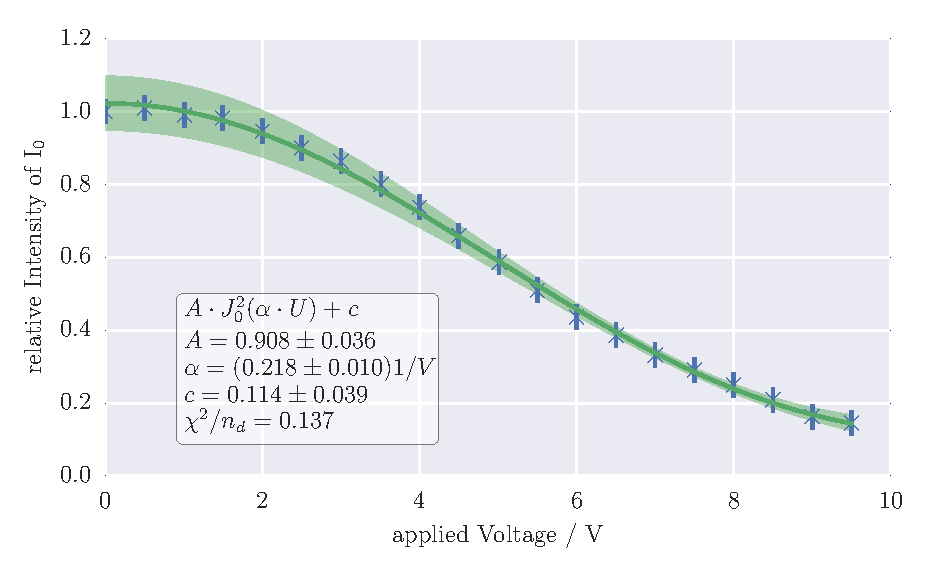
\includegraphics[width=1\textwidth]{analysis/figures/besselfit_000}
    \caption{The measurements and the least square fit with the maxima of order zero. 
    The error bars are given by 3\% of the extent of the oscilloscope,
    while the light green surface is the upper and lower limit of the fitted function, calculated 
    with the covariance matrix of the coefficients. 
    We fit the data with the function derived in the theoretical
    section, but extent it by an factor $c$ in order to take into account an additional (constant) noise
    influencing the photo diodes. 
    \\
    $\Rightarrow$ We notice the agreement of our measurements with the Raman-Nath theory. Using the
    coefficient $\alpha$ from the fit we will calculate the sonic wave length in the following section.}
    \label{fig:besselfit_000}
\end{figure}
\begin{SCfigure}
\caption{
The covariance matrix of the coefficients, calculated by the least square method. The off-diagonals are
one order of magnitude less than the errors, except for the releation between $A$ and $c$, which accounts for the
uncertainty of the estimated background. Keeping in mind that an higher background would lead to a smaller
amplitude (given the same data) we notice that the absolute error of $A$ and $c$ is much higher than the error for $\alpha$.
}
 \begin{tabular}{|r|r|r|r|}
 \hline 
\cellcolor{tabcolor}&\cellcolor{tabcolor}$\alpha$&\cellcolor{tabcolor}$A$&\cellcolor{tabcolor}$c$\\ \hline 
 \cellcolor{tabcolor}$\alpha$&$0.00010$ &$-0.00028$ &$0.00036$ \\ 
\cellcolor{tabcolor}$A$&$-0.00028$ &$0.00132$ &$-0.00130$ \\ 
\cellcolor{tabcolor}$c$&$0.00036$ &$-0.00130$ &$0.00151$ \\ \hline \hline
\cellcolor{tabcolor}$\alpha$&\multicolumn{3}{r|}{$0.21839 \pm 0.00989$ }\\ 
\cellcolor{tabcolor}$A$&\multicolumn{3}{r|}{$0.90833 \pm 0.03628$ }\\ 
\cellcolor{tabcolor}$c$&\multicolumn{3}{r|}{$0.11427 \pm 0.03881$ }\\ 
\hline\end{tabular}
\end{SCfigure}

\newpage

\begin{figure}[htpb]
    \centering
    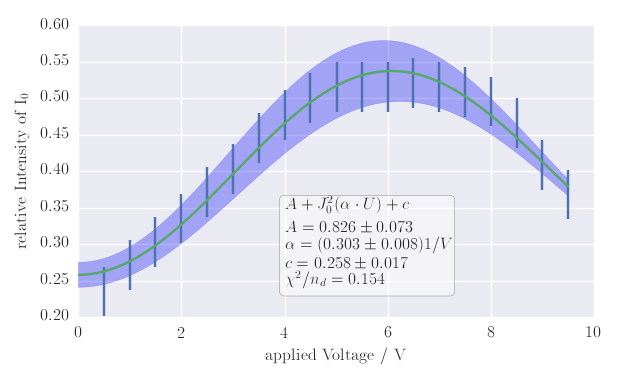
\includegraphics[width=1\textwidth]{analysis/figures/besselfit_001}
    \caption{
        The measurements and the least square fit with the maxima of first order, where
        the maxima were calculated with $I = (I_{\mathrm{left}} +  I_{\mathrm{right}})/2$.
        For further details on the applied procedure, see for figure~\ref{fig:besselfit_000}.
        Additionally we notice that the method estimating the maxima is encumbered by the 
        bad resolution of the peaks itself, such that they are not separated as they should. 
        Following from this we receive a huge systematic error, not being reflected in the
        statistical errors resulting from the least squares fit. \\
        $\Rightarrow$ The important characteristic value $\alpha$ disagrees 
        with the result of the maxima of zeroth order, which
        should in theory be the same. Noting that the $\chi^2$ test is lower then 1 (which would rather indicate that
        the given errors are too small or the hypothesis is wrong) we remark that the 
        systematic errors have an huge impact on the result, reflecting
        also in the disagreement within the parameters $A$ and $c$. 
        }
    \label{fig:besselfit_001}
\end{figure}


\begin{SCfigure}
    \caption{
        As before, only $A$ and $c$ are coupled, which is also visible in the
        bigger error. Since $\alpha$ is (according to the least squares fit)
        independent of the others, the systematic error described before (see caption of figure~\ref{fig:besselfit_001}) 
        cannot depend on the amplitude or a constant background noise alone, 
        but has to be related to the increased curvature
        visible in an higher $\alpha$.}
    \begin{tabular}{|r|r|r|r|}
        \hline 
        \cellcolor{tabcolor}&\cellcolor{tabcolor}$\alpha$&\cellcolor{tabcolor}$A$&\cellcolor{tabcolor}$c$\\ \hline 
        \cellcolor{tabcolor}$\alpha$&$0.00006$ &$-0.00004$ &$-0.00000$ \\ 
        \cellcolor{tabcolor}$A$&$-0.00004$ &$0.00532$ &$-0.00110$ \\ 
        \cellcolor{tabcolor}$c$&$-0.00000$ &$-0.00110$ &$0.00029$ \\ \hline \hline
        \cellcolor{tabcolor}$\alpha$&\multicolumn{3}{r|}{$0.30305 \pm 0.00792$ }\\ 
        \cellcolor{tabcolor}$A$&\multicolumn{3}{r|}{$0.82599 \pm 0.07293$ }\\ 
        \cellcolor{tabcolor}$c$&\multicolumn{3}{r|}{$0.25782 \pm 0.01709$ }\\ 
        \hline
    \end{tabular}
\end{SCfigure}
\newpage
\begin{figure}[htpb]
    \centering
    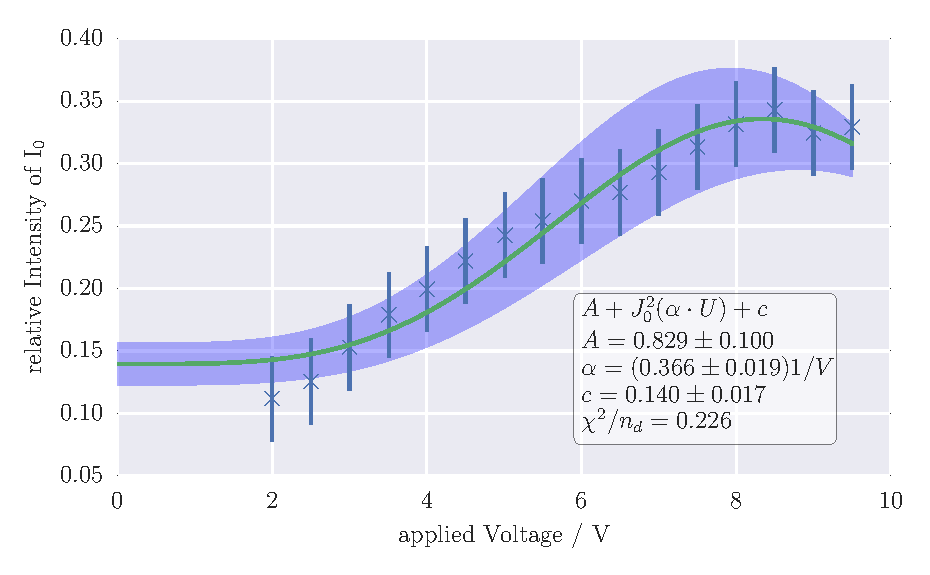
\includegraphics[width=1\textwidth]{analysis/figures/besselfit_002}
    \caption{This is the fit of the maxima of second order. For
    introductory remarks please see figure~\ref{fig:besselfit_000} and figure~\ref{fig:besselfit_001}.
    Again, as already observed in the maxima of first order, the curvature $\alpha$ has increased again.
    We want to emphasize the fact that the unreliability of this analysis is very low, because of \\
    \textbf{a) the low resolution} of the peaks such that they were not clearly separated 
    from the other maxima.\\
    \textbf{b) the strong disagreement} of $\alpha$ with the result of the other maxima, 
    further indicating to the systematic error.   
    }
    \label{fig:besselfit_002}
\end{figure}

\begin{SCfigure}
\caption{
    Since the fit is not reliable (as mentioned in figure~\ref{fig:besselfit_002}), 
    the covariance matrix along with the errors cannot have further significance.
    We note that the errors are too small to take into account the strong deviation to the
    other results. They should be corrected with an inherent systematic error, as considered in
    the remarks of figure~\ref{fig:besselfit_000} and figure~\ref{fig:besselfit_001}.
}
 \begin{tabular}{|r|r|r|r|}
 \hline 
\cellcolor{tabcolor}&\cellcolor{tabcolor}$\alpha$&\cellcolor{tabcolor}$A$&\cellcolor{tabcolor}$c$\\ \hline 
 \cellcolor{tabcolor}$\alpha$&$0.00037$ &$0.00028$ &$-0.00013$ \\ 
\cellcolor{tabcolor}$A$&$0.00028$ &$0.00992$ &$-0.00137$ \\ 
\cellcolor{tabcolor}$c$&$-0.00013$ &$-0.00137$ &$0.00029$ \\ \hline \hline
\cellcolor{tabcolor}$\alpha$&\multicolumn{3}{r|}{$0.36608 \pm 0.01934$ }\\ 
\cellcolor{tabcolor}$A$&\multicolumn{3}{r|}{$0.82888 \pm 0.09961$ }\\ 
\cellcolor{tabcolor}$c$&\multicolumn{3}{r|}{$0.13956 \pm 0.01695$ }\\ 
\hline
\end{tabular}
\end{SCfigure}
\newpage
\clearpage
\begin{figure}[htpb]
    \centering
    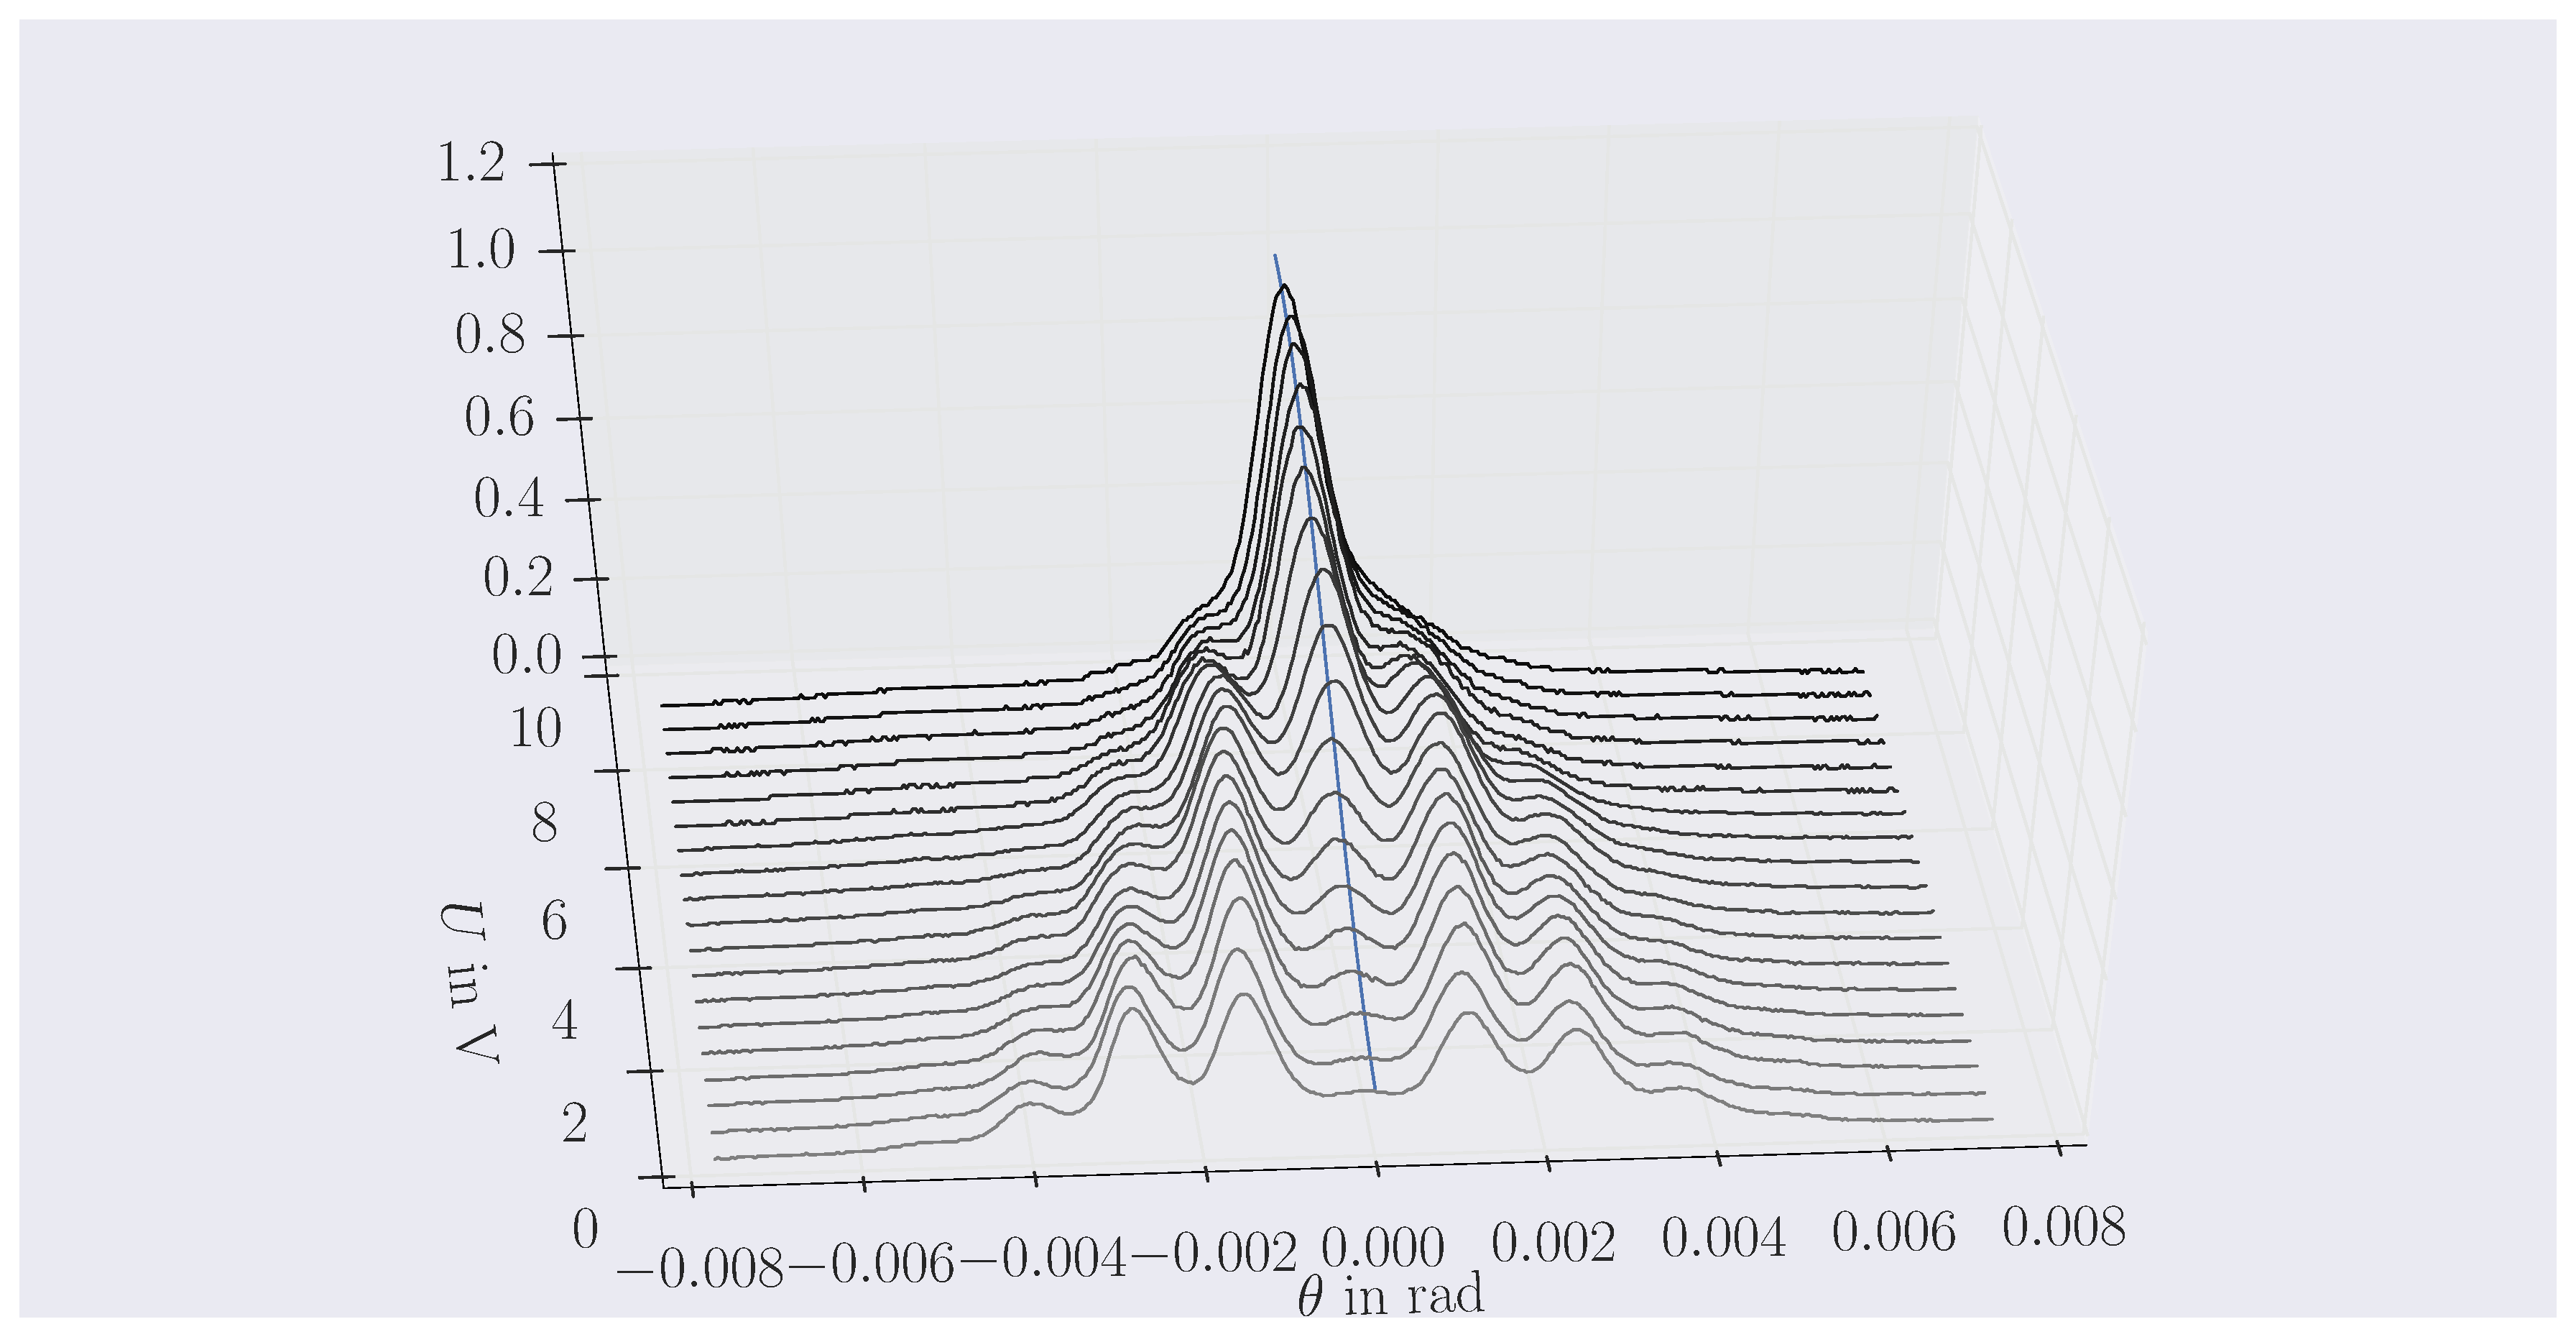
\includegraphics[width=1\textwidth]{./figures/plot3d}
    \caption{   Visualization of the measurements with 3d projection.
    }
    \label{fig:plot3d}
\end{figure}


\subsubsection{Sonic wave length}
As far as we can consider the results of our measurements,
we can estimate the sonic wave length with the already
given equation 
\begin{equation}
\sin(\theta_m) = \frac{m \lambda}{\Lambda}.
\end{equation}
We notice that the estimated value is not constant for all voltages, unlike as predicted by theory; 
see figure~\ref{fig:soundspeed} for the discrepancy of estimating $\Lambda$ with the maxima 
of first order for different $U$.
We suspect this to be due mostly to the described shortcomings in resolution. 
However, we note other systematical errors might be induced by other 
electro-optical effects such as dispersion. The instability of frequency generation
seems to be of negligible order.
\begin{figure}[H]
    \centering
    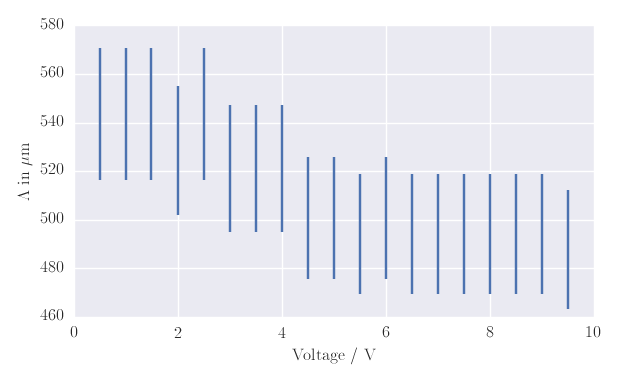
\includegraphics[width=1\textwidth]{analysis/figures/soundspeed}
    \caption{
        These are the estimated values for $\Lambda$ with regards to the maxima of first order.
        We notice that the wavelength is not constant for all voltages. The error bar is given by
        gaussian error propagation of the uncertainty in finding the position of the maxima (the
        width of the maximum).}
    \label{fig:soundspeed}
\end{figure}
The mean value of the values for maxima of first order yields
\begin{equation}
    \Lambda = \left [511 \pm 26 \right ]\, \mu\mathrm{m}.
\end{equation}
In order to judge the quality of this estimation we can alternatively calculate the
wavelength with the sonic speed in Isooctane $c = 1111\,$m/s (given in \cite{staatsexamen})
and the 
frequency of the piezoelectric crystal $f =2132 \pm 5\,$Hz (where the uncertainty is given
by the unstable signal we measured over the whole experiment):
\begin{equation}
\Lambda = \frac{c}{f} = \left [521 \pm 1 \right ] \mu m
\end{equation}
Despite all difficulties discussed before, our prior estimation 
lies in this more precise value within the stated error. 
We thus conclude that at least for the first maximum, 
the obtained data can be used for the calculation. 
This further underlines the agreement of Raman-Nath theory
with the observations.
which is within the range of our former estimation. 


\clearpage

\section{Bibliography}
\printbibliography[heading=subbibintoc,type=article,title={Articles}]
\printbibliography[heading=subbibintoc,type=book,title={Books}]
\printbibliography[heading=subbibintoc,type=misc,title={Other}]
\clearpage
\section{Appendix: Handwritten records of the experiment}
\label{sec:appendix}
    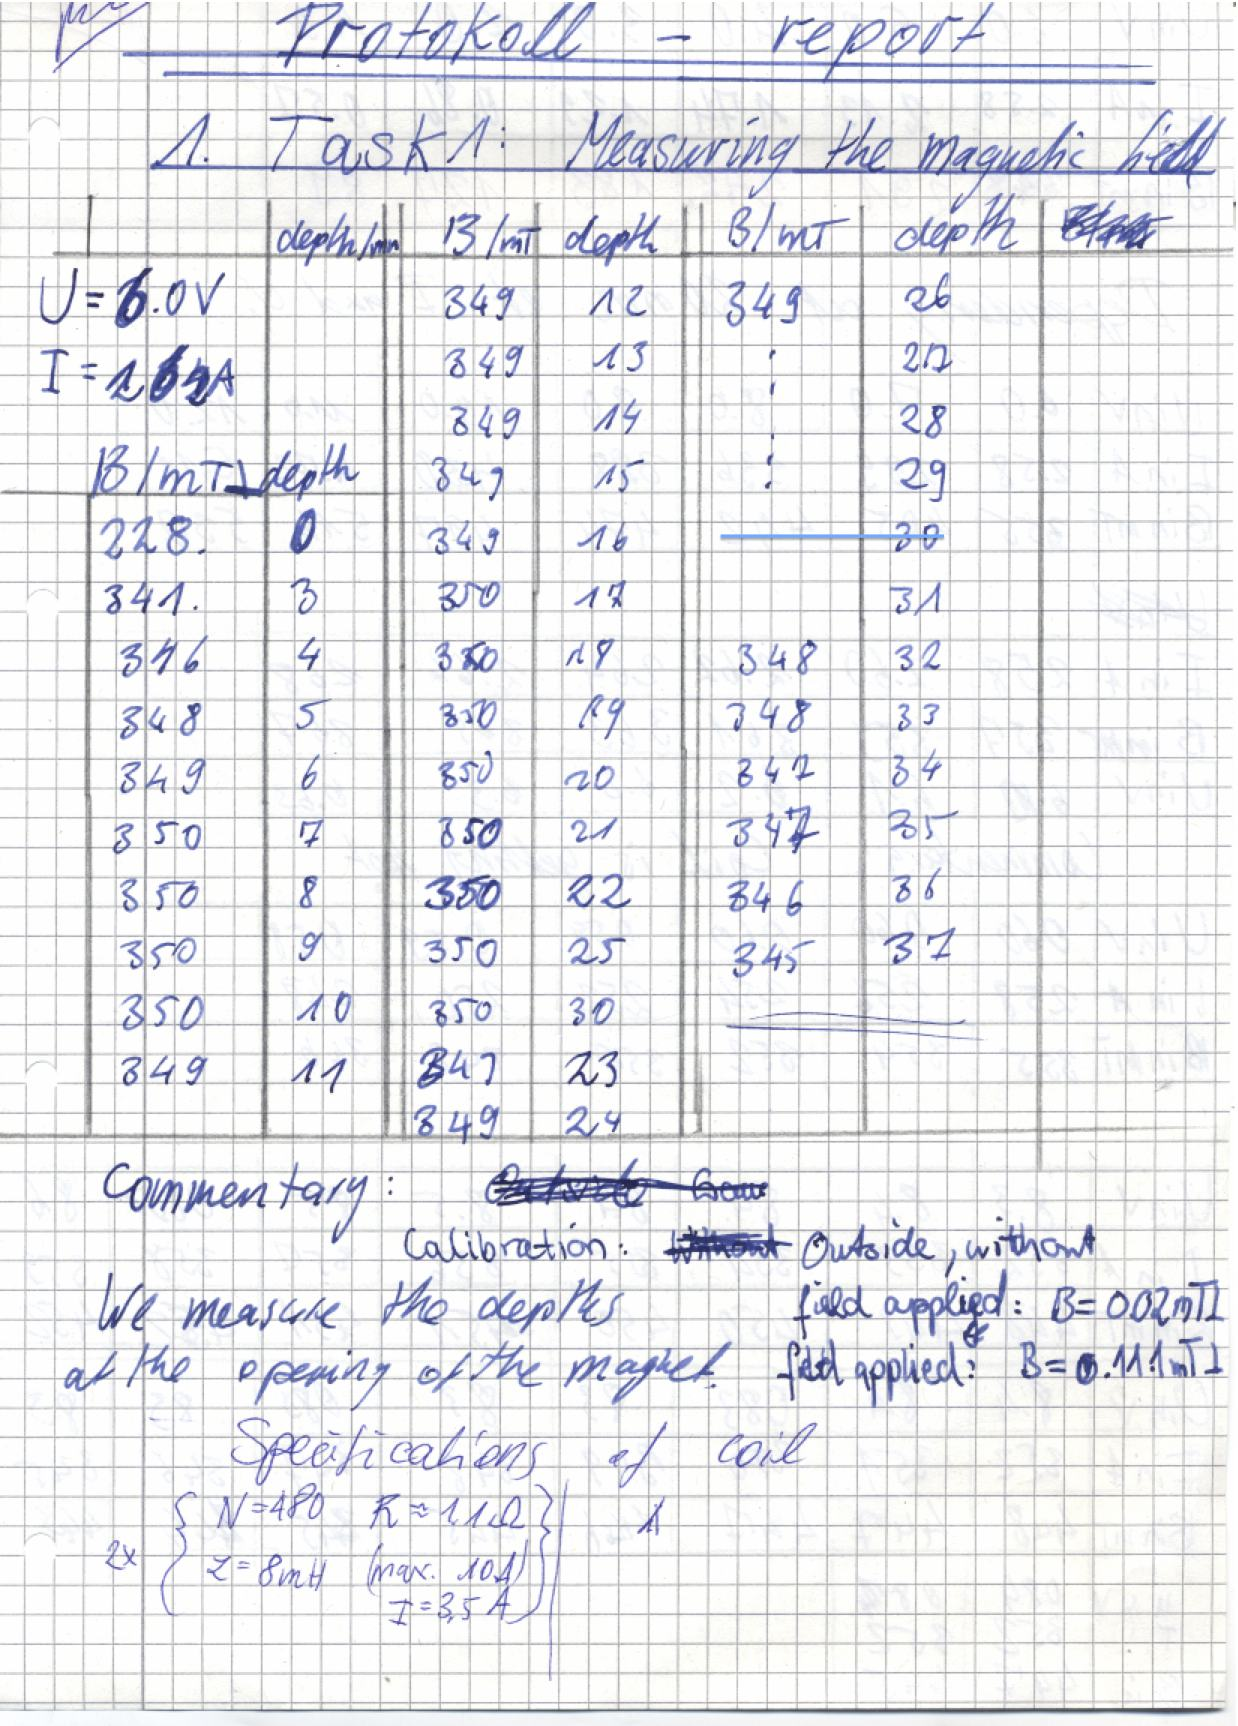
\includegraphics[width=\linewidth]{appendix/spin1.jpg}
\clearpage
    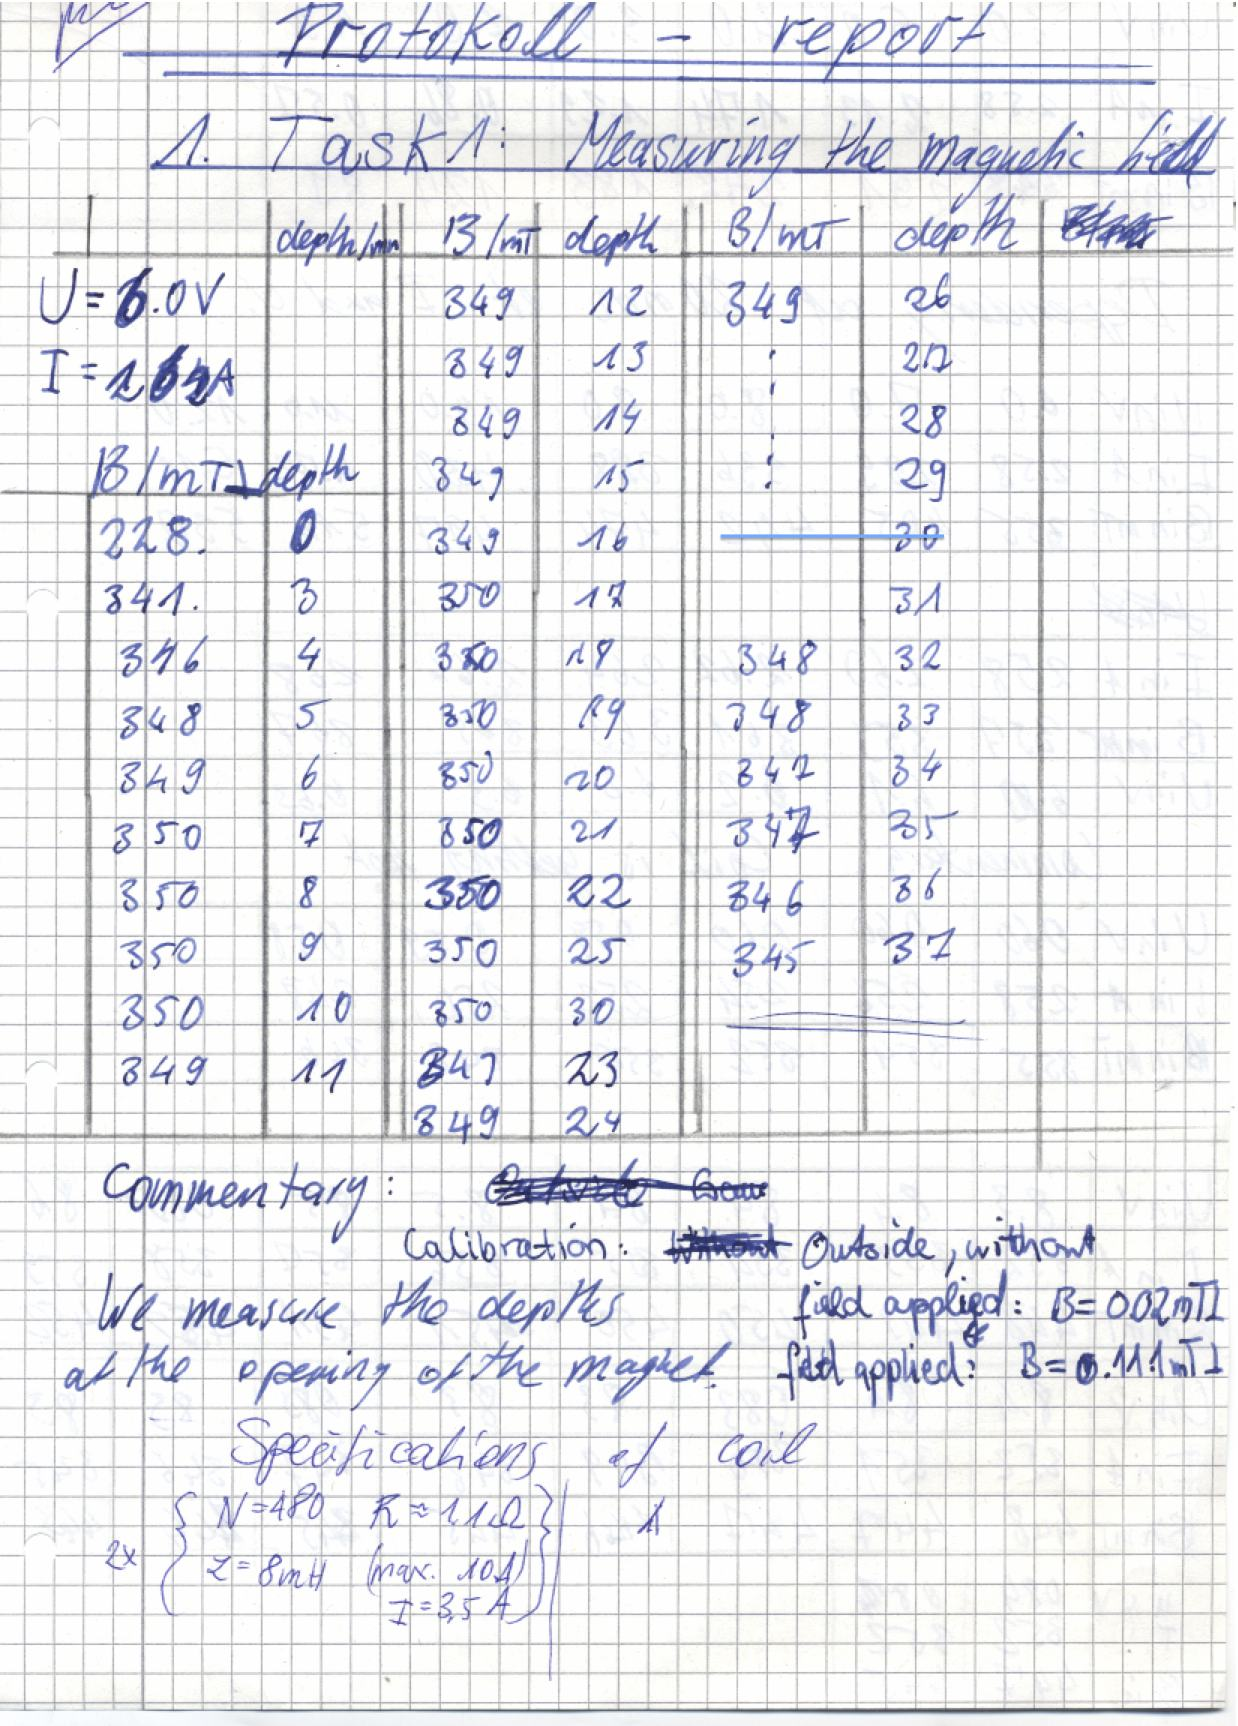
\includegraphics[width=\linewidth]{appendix/spin1.jpg}
\clearpage
    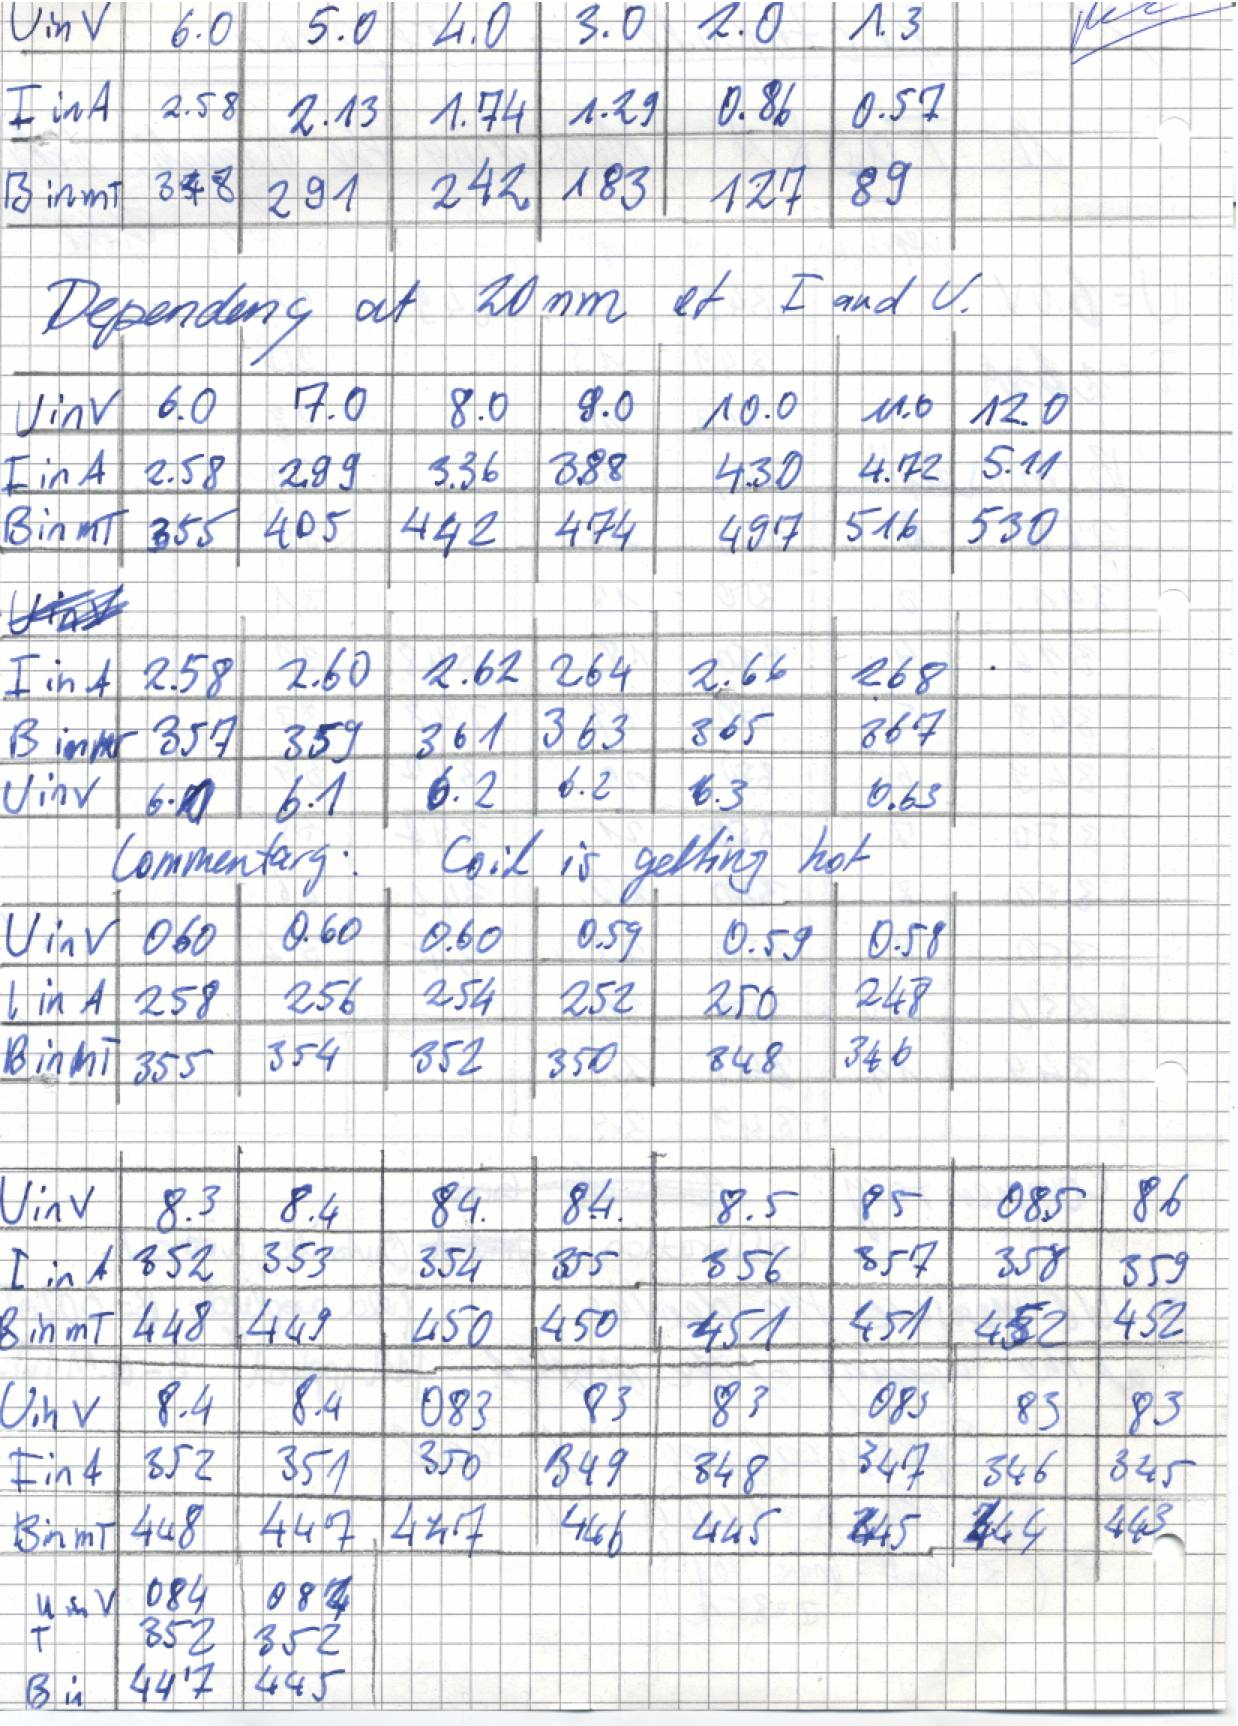
\includegraphics[width=\linewidth]{appendix/spin2.jpg}
\clearpage
    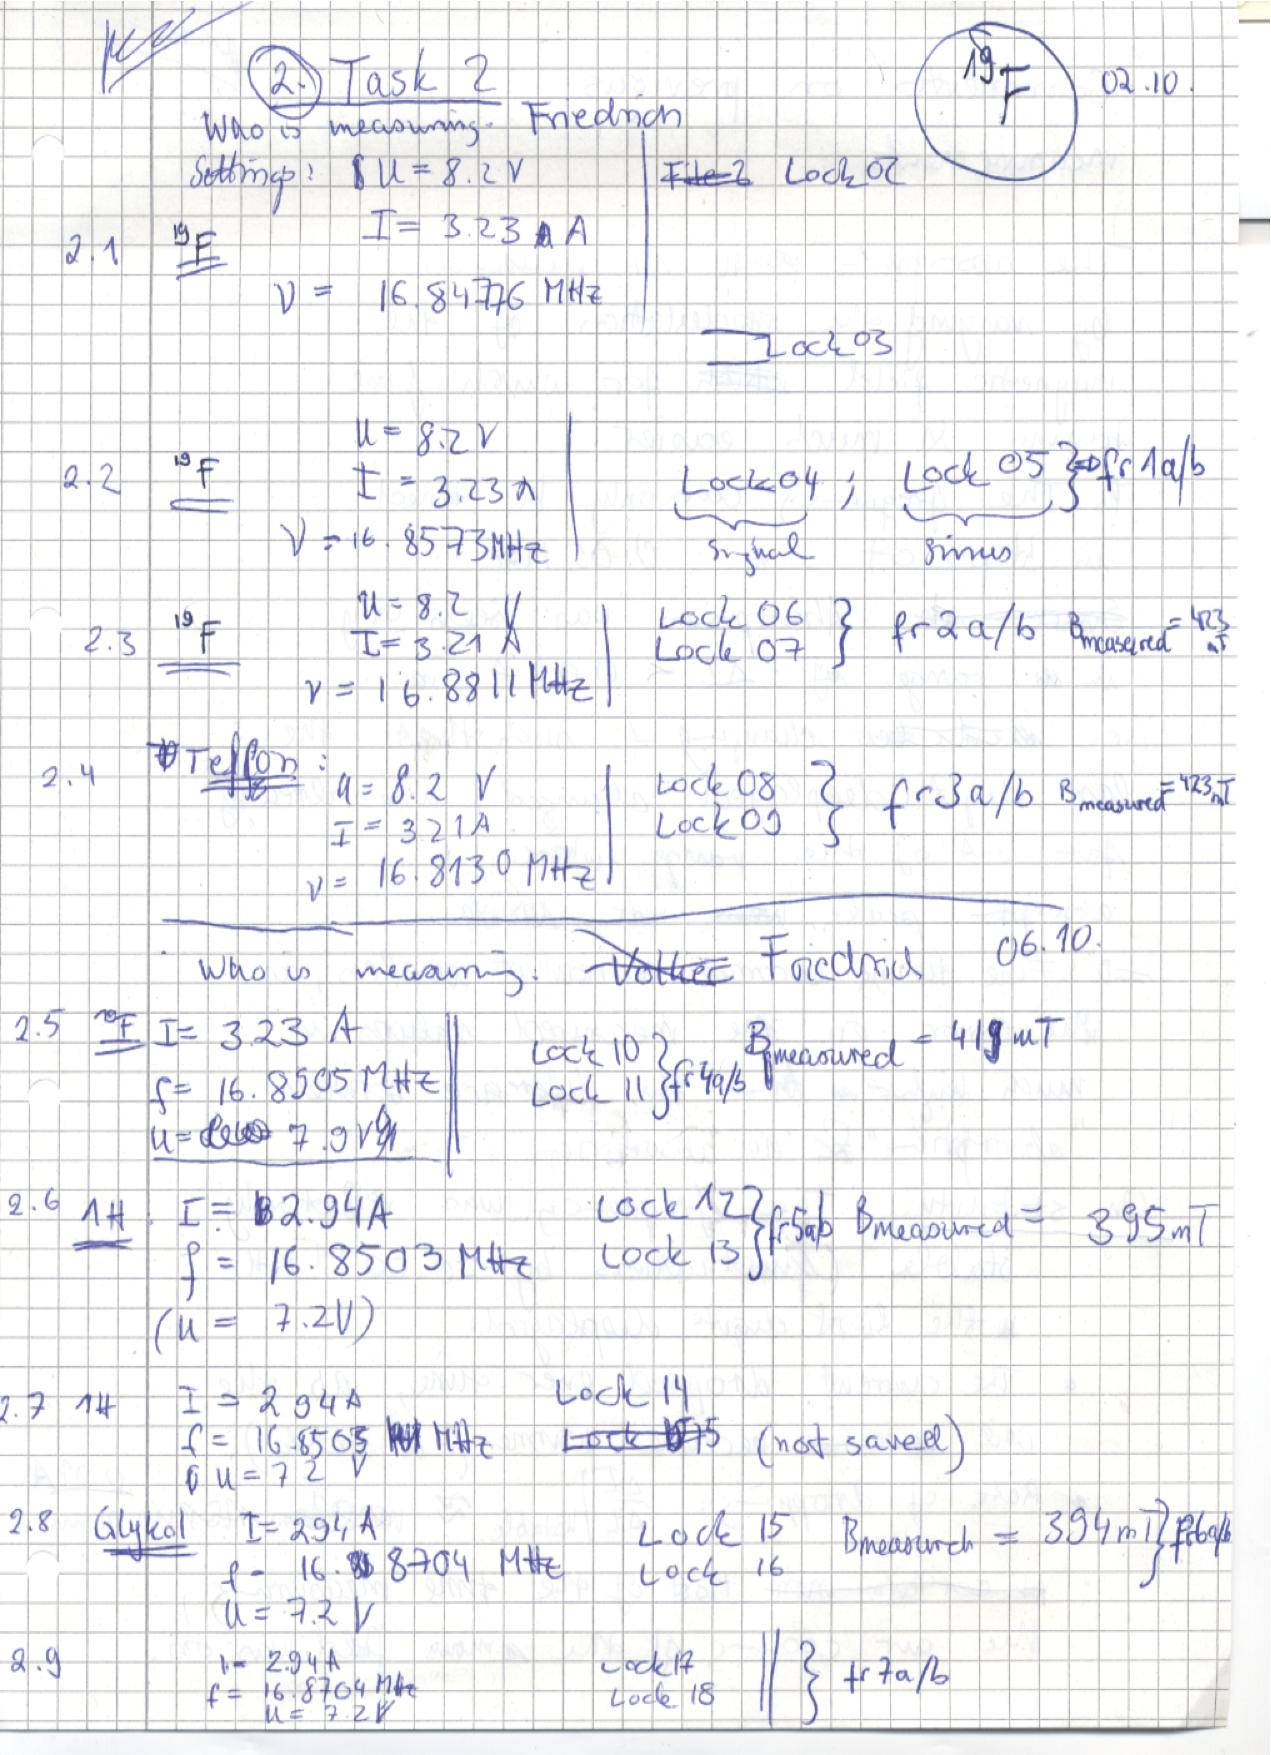
\includegraphics[width=\linewidth]{appendix/spin3.jpg}
\clearpage
    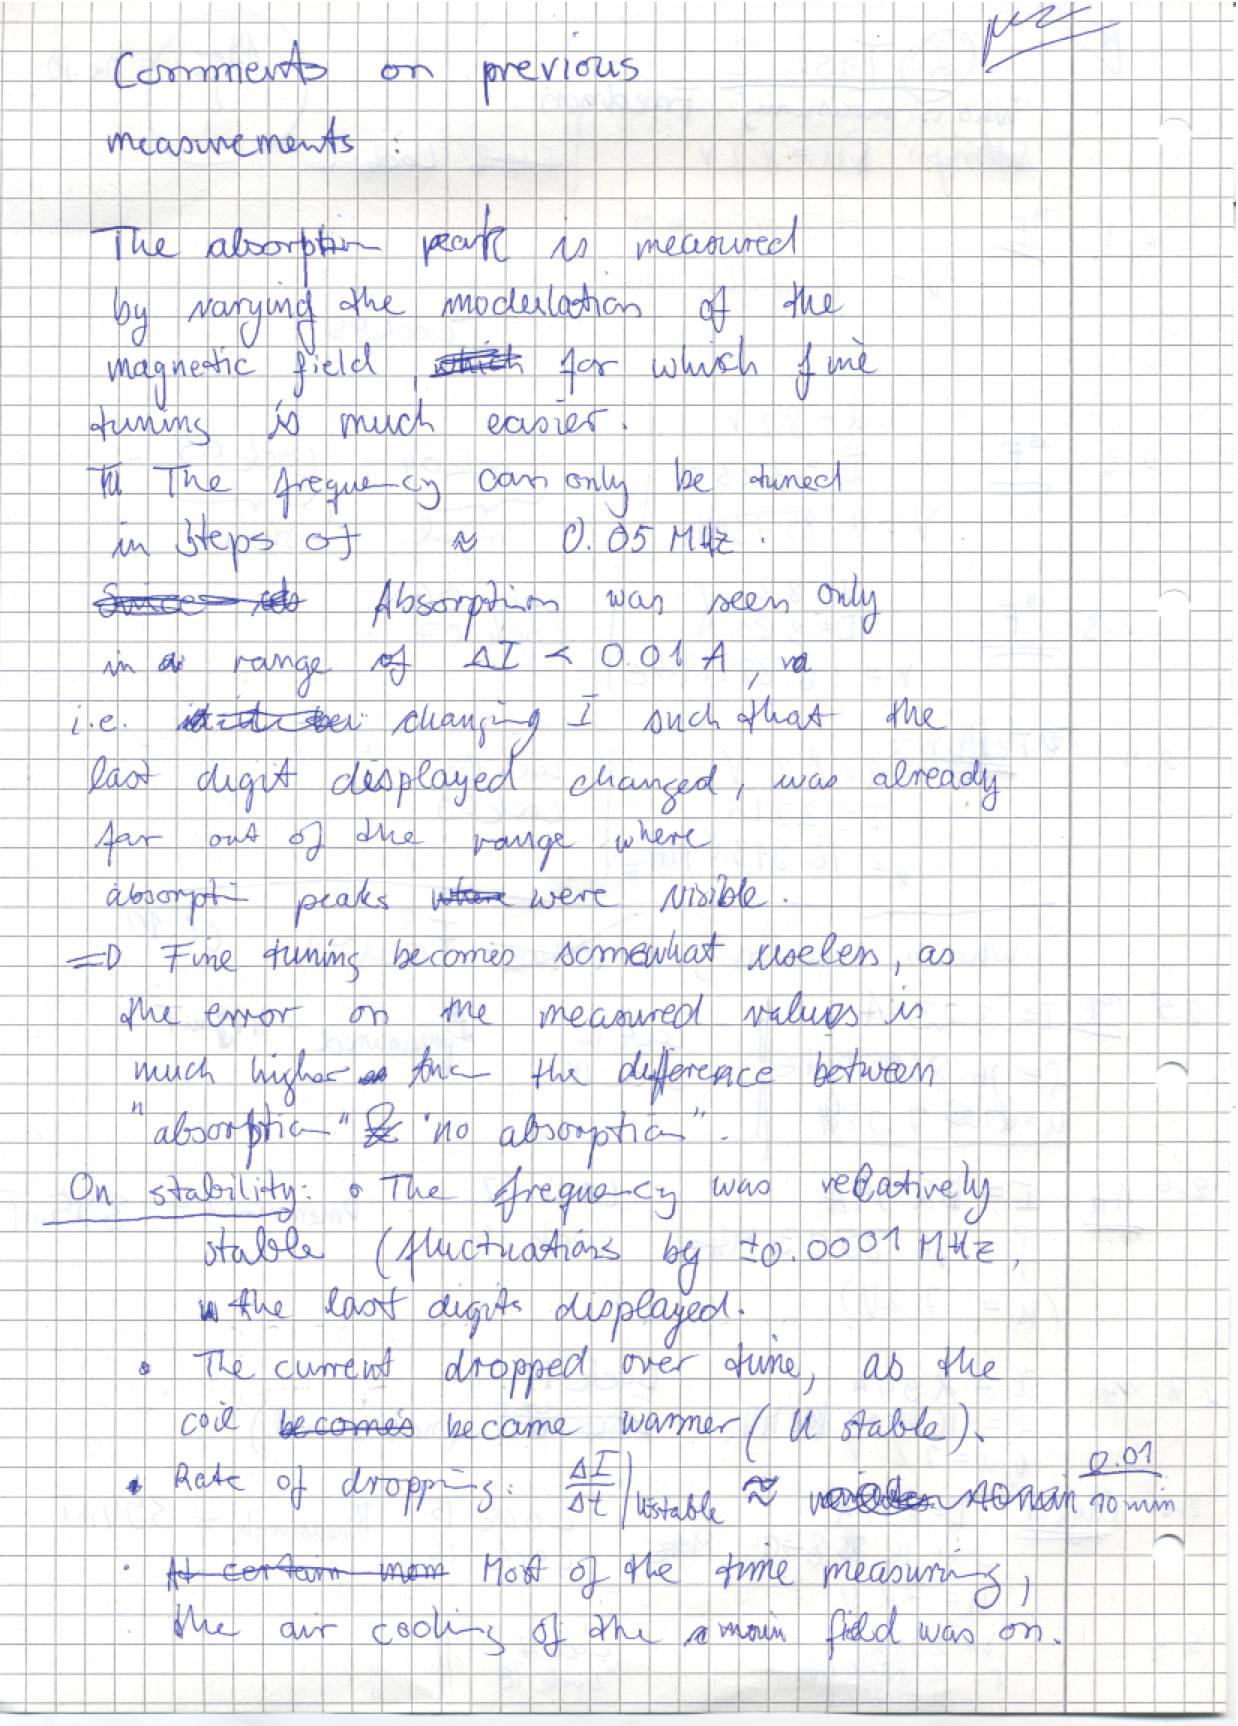
\includegraphics[width=\linewidth]{appendix/spin4.jpg}
\clearpage
    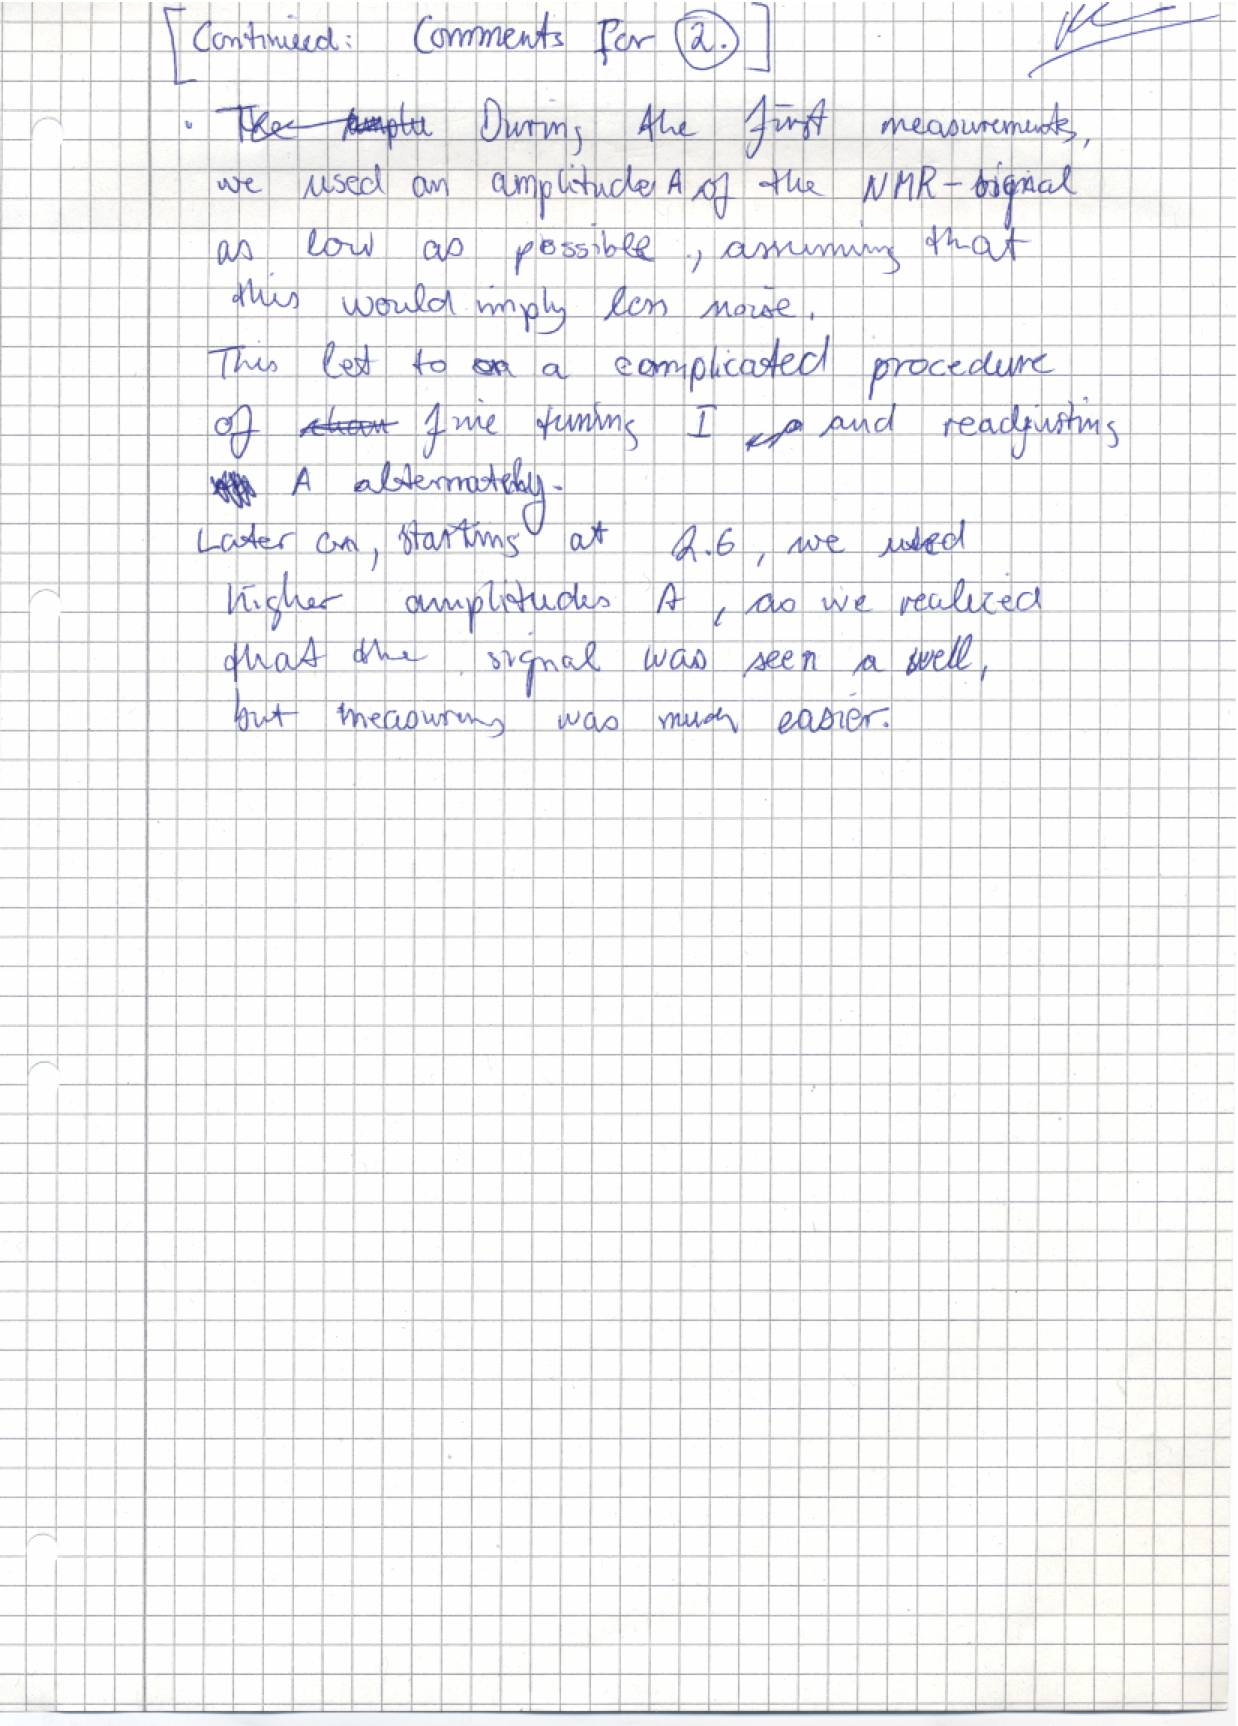
\includegraphics[width=\linewidth]{appendix/spin5.jpg}
\clearpage
    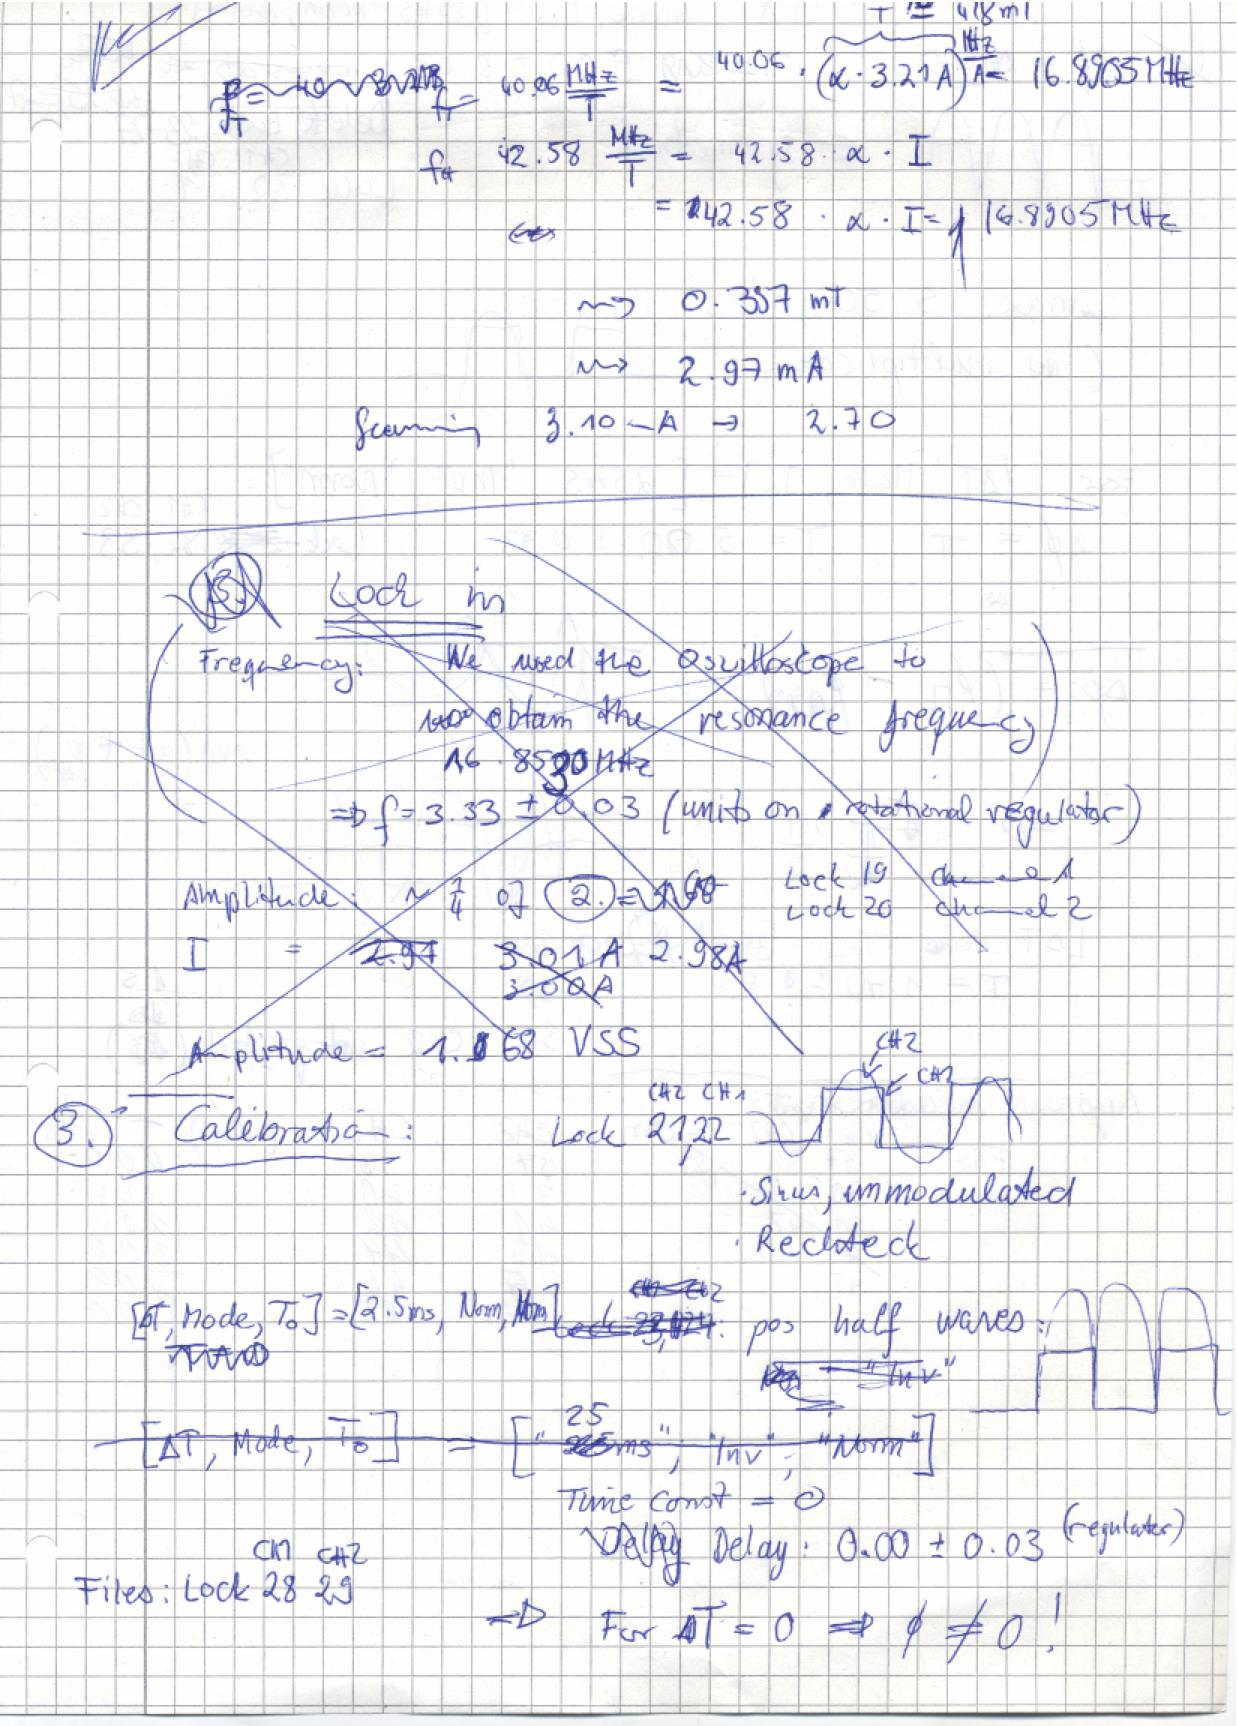
\includegraphics[width=\linewidth]{appendix/spin6.jpg}
\clearpage
    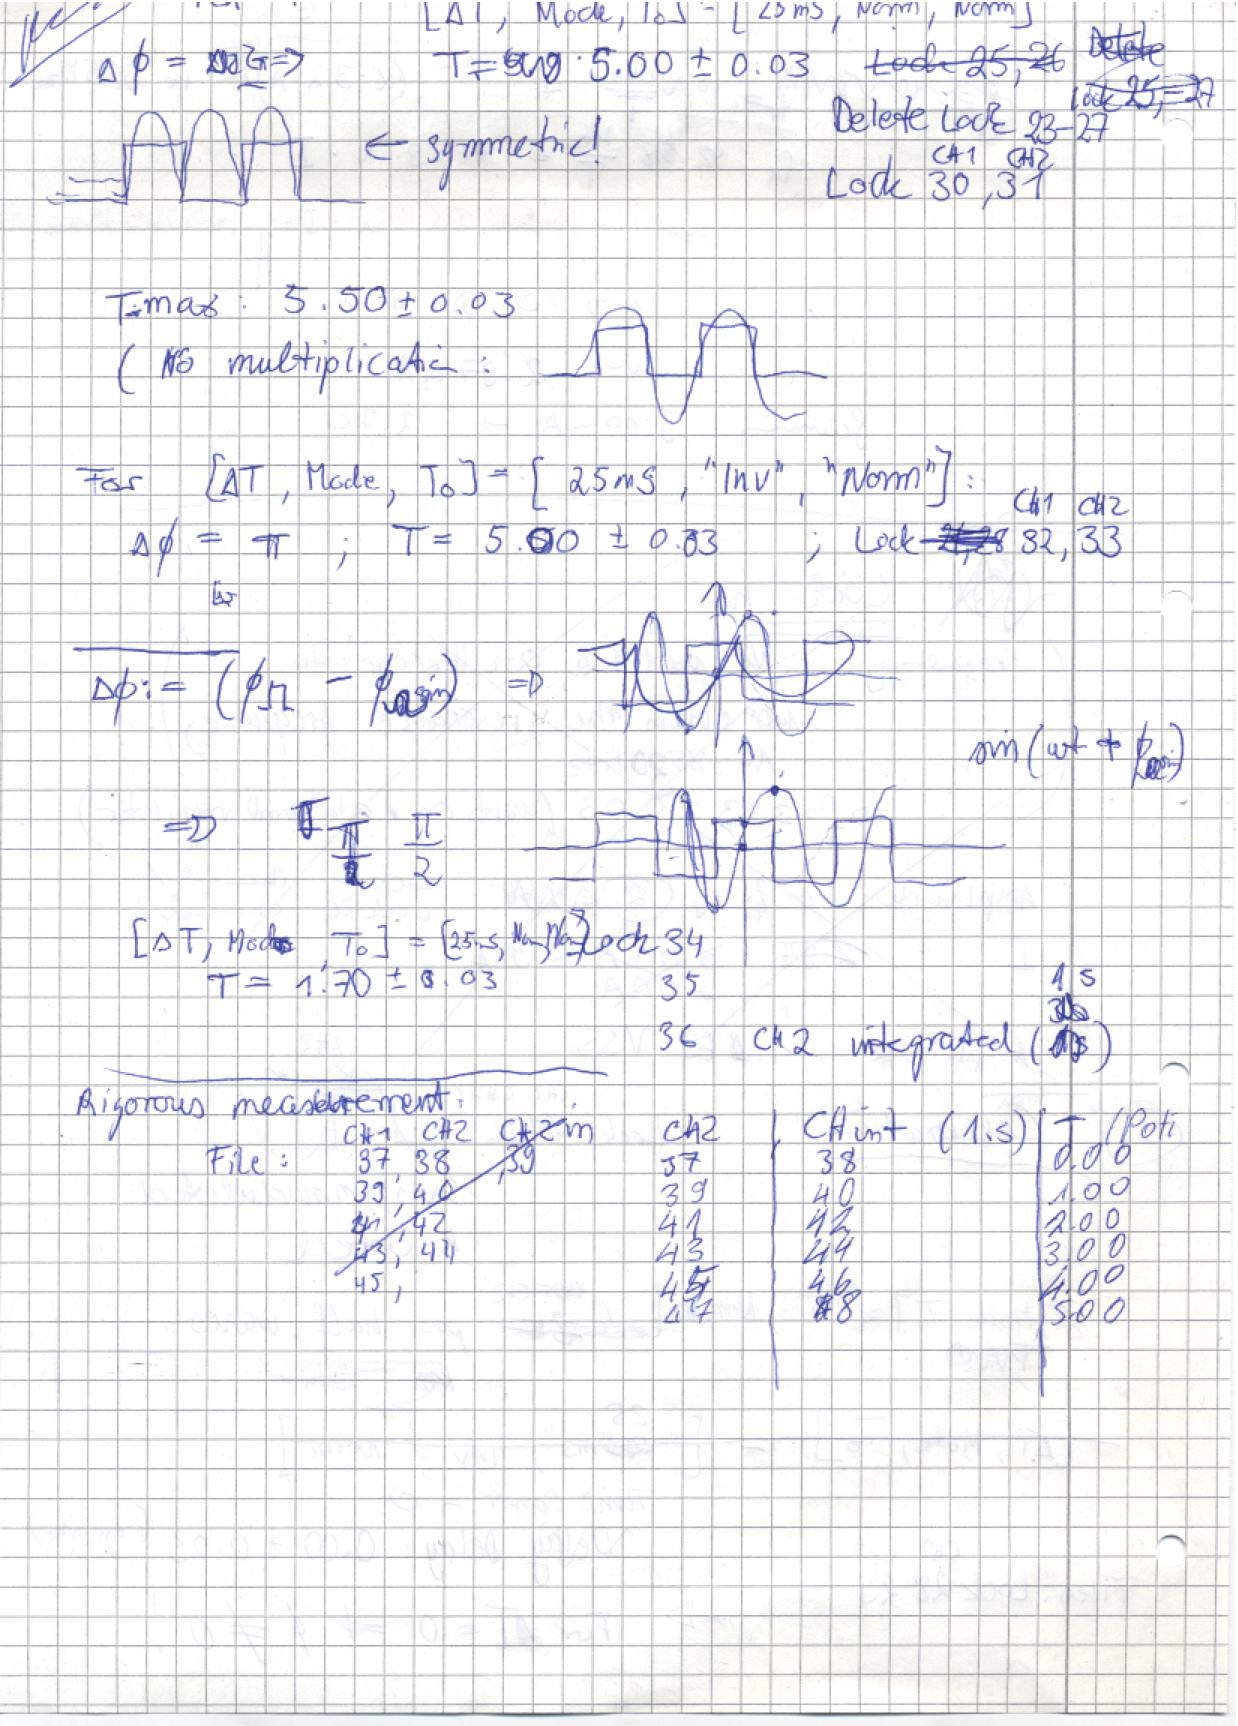
\includegraphics[width=\linewidth]{appendix/spin7.jpg}
\clearpage



\end{document}
